\chapter{Supervised learning \& generalization}
\section{Backpropagation in feedforward multi-layer networks}
In this exercise we train a feed forward neural network to fit the function $y = sin(x^2)$ with and without noise. The universal approximation theorem states that under mild activation assumptions a feed forward neural network with a single hidden layer and finite number of neurons can approximate a continuous function well. Therefore, we train a network with single hidden layer and evaluate the performance using various training algorithms like gradient descent \textit{(traingd)}, gradient descent with adaptive learning rate \textit{(traingda)}, Fletcher-Reeves conjugate gradient \textit{(traincgf )}, Polak-Ribiere
conjugate gradient \textit{(traincgp)}, BFGS quasi Newton \textit{(trainbfg)}, Levenberg-Marquardt \textit{(trainlm)} and Levenberg-Marquardt with Bayesian regularization \textit{(trainbr)}. We compare the results of these algorithms with gradient descent. The function approximations of these algorithms trained for 1000 epochs is shown in the below figure \ref{fig:train_gd}. 
\begin{figure}[ht]
	\begin{subfigure}[b]{0.33\textwidth}
		\centering
		\captionsetup{ width=0.8\linewidth, format = hang}
		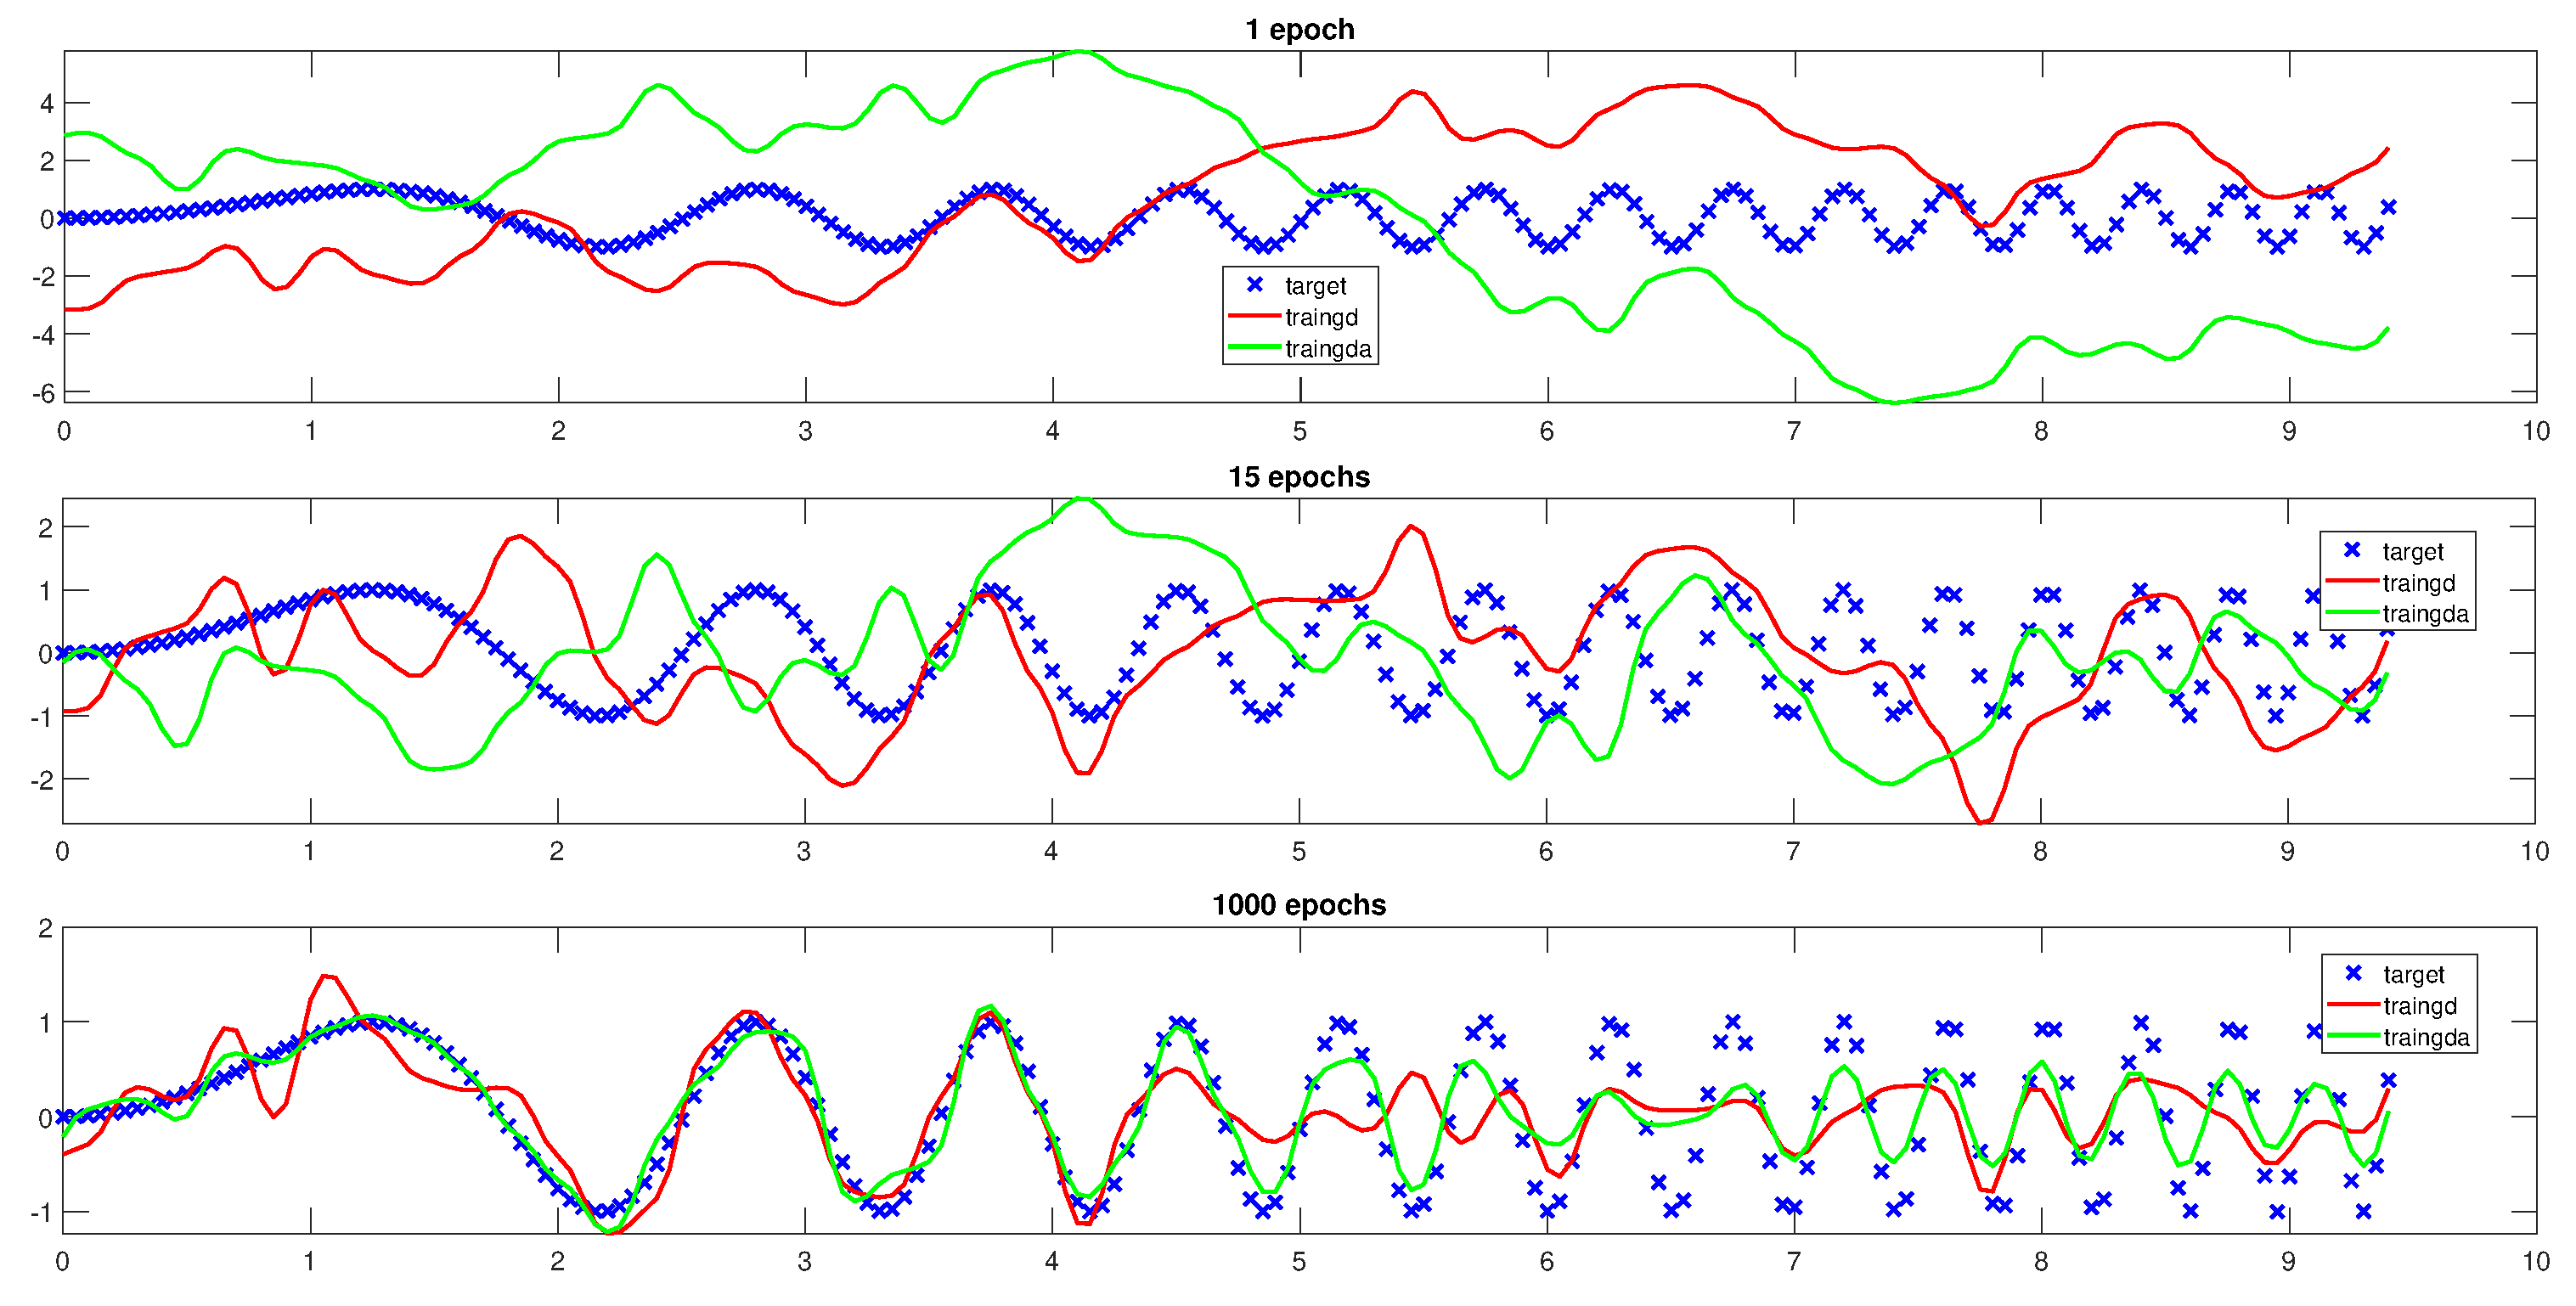
\includegraphics[height = 0.7\textwidth, width = 1\textwidth]{Exercise1/Report/train_gd_gda}
		\caption{train\_gd VS train\_gda}\label{fig:train_gd_gda}
	\end{subfigure}%
	\begin{subfigure}[b]{0.33\textwidth}
		\centering
		\captionsetup{width=0.8\linewidth, format = hang}
		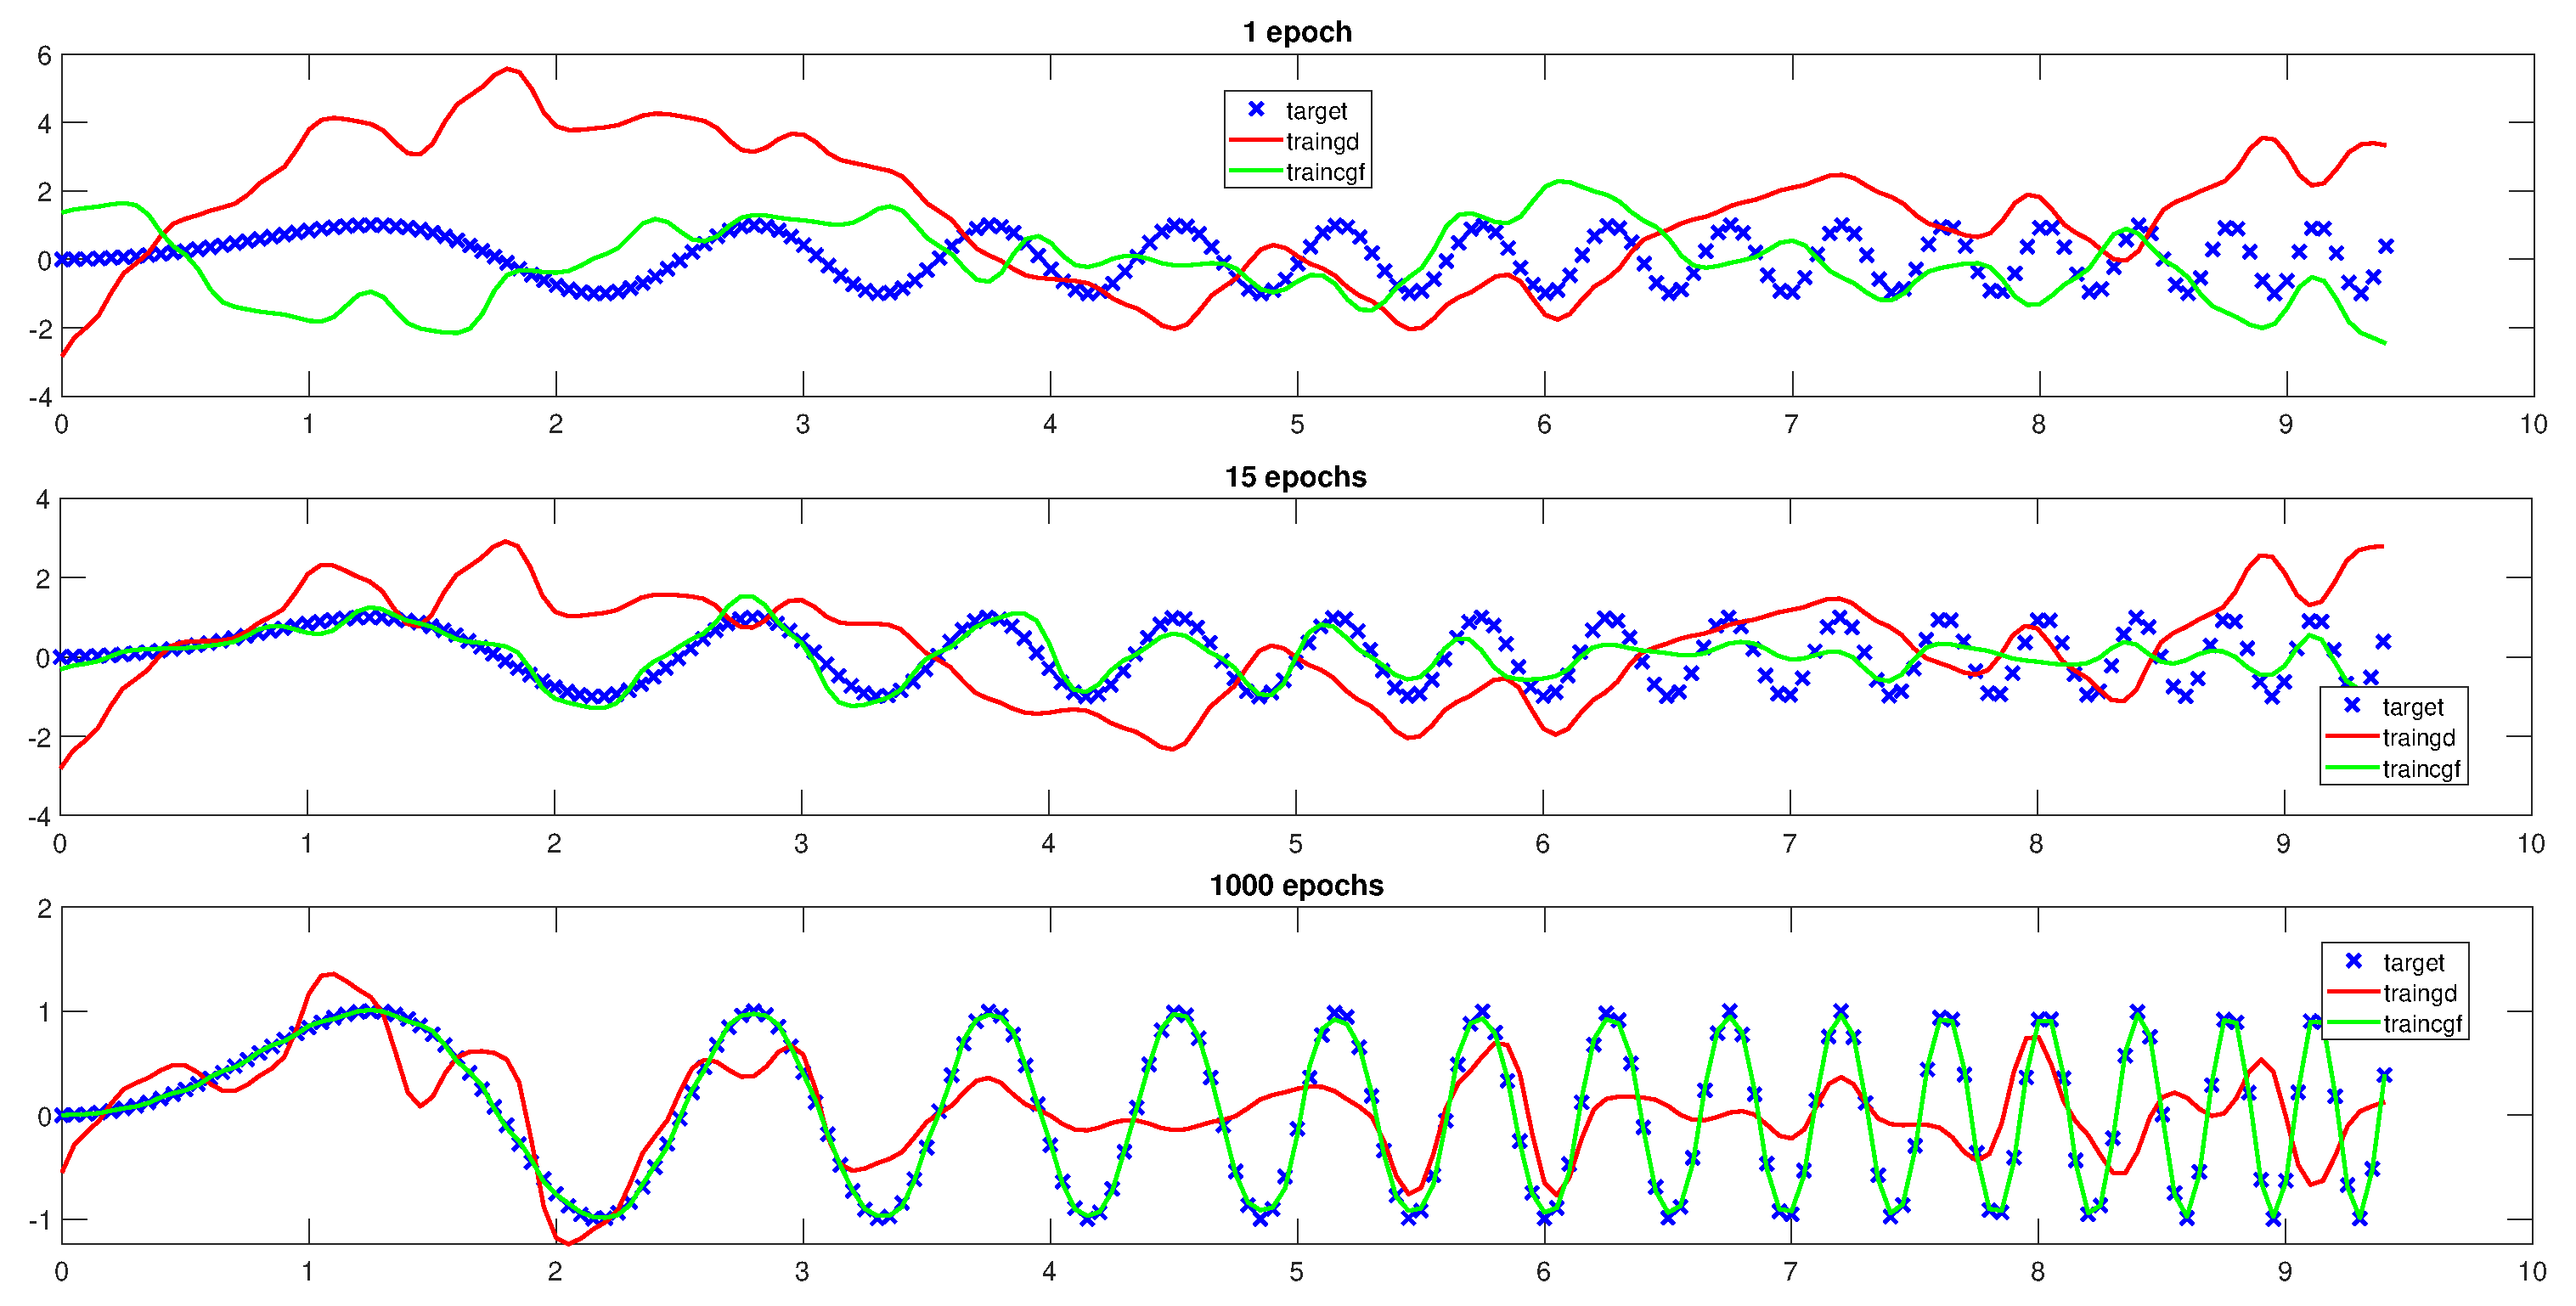
\includegraphics[height = 0.7\textwidth, width = 1\textwidth]{Exercise1/Report/train_gd_cgf}
		\caption{train\_gd VS  train\_cgf}\label{fig:train_gd_cgf}
	\end{subfigure}%
	\begin{subfigure}[b]{0.33\textwidth}
		\centering
		\captionsetup{width=0.8\linewidth, format = hang}
		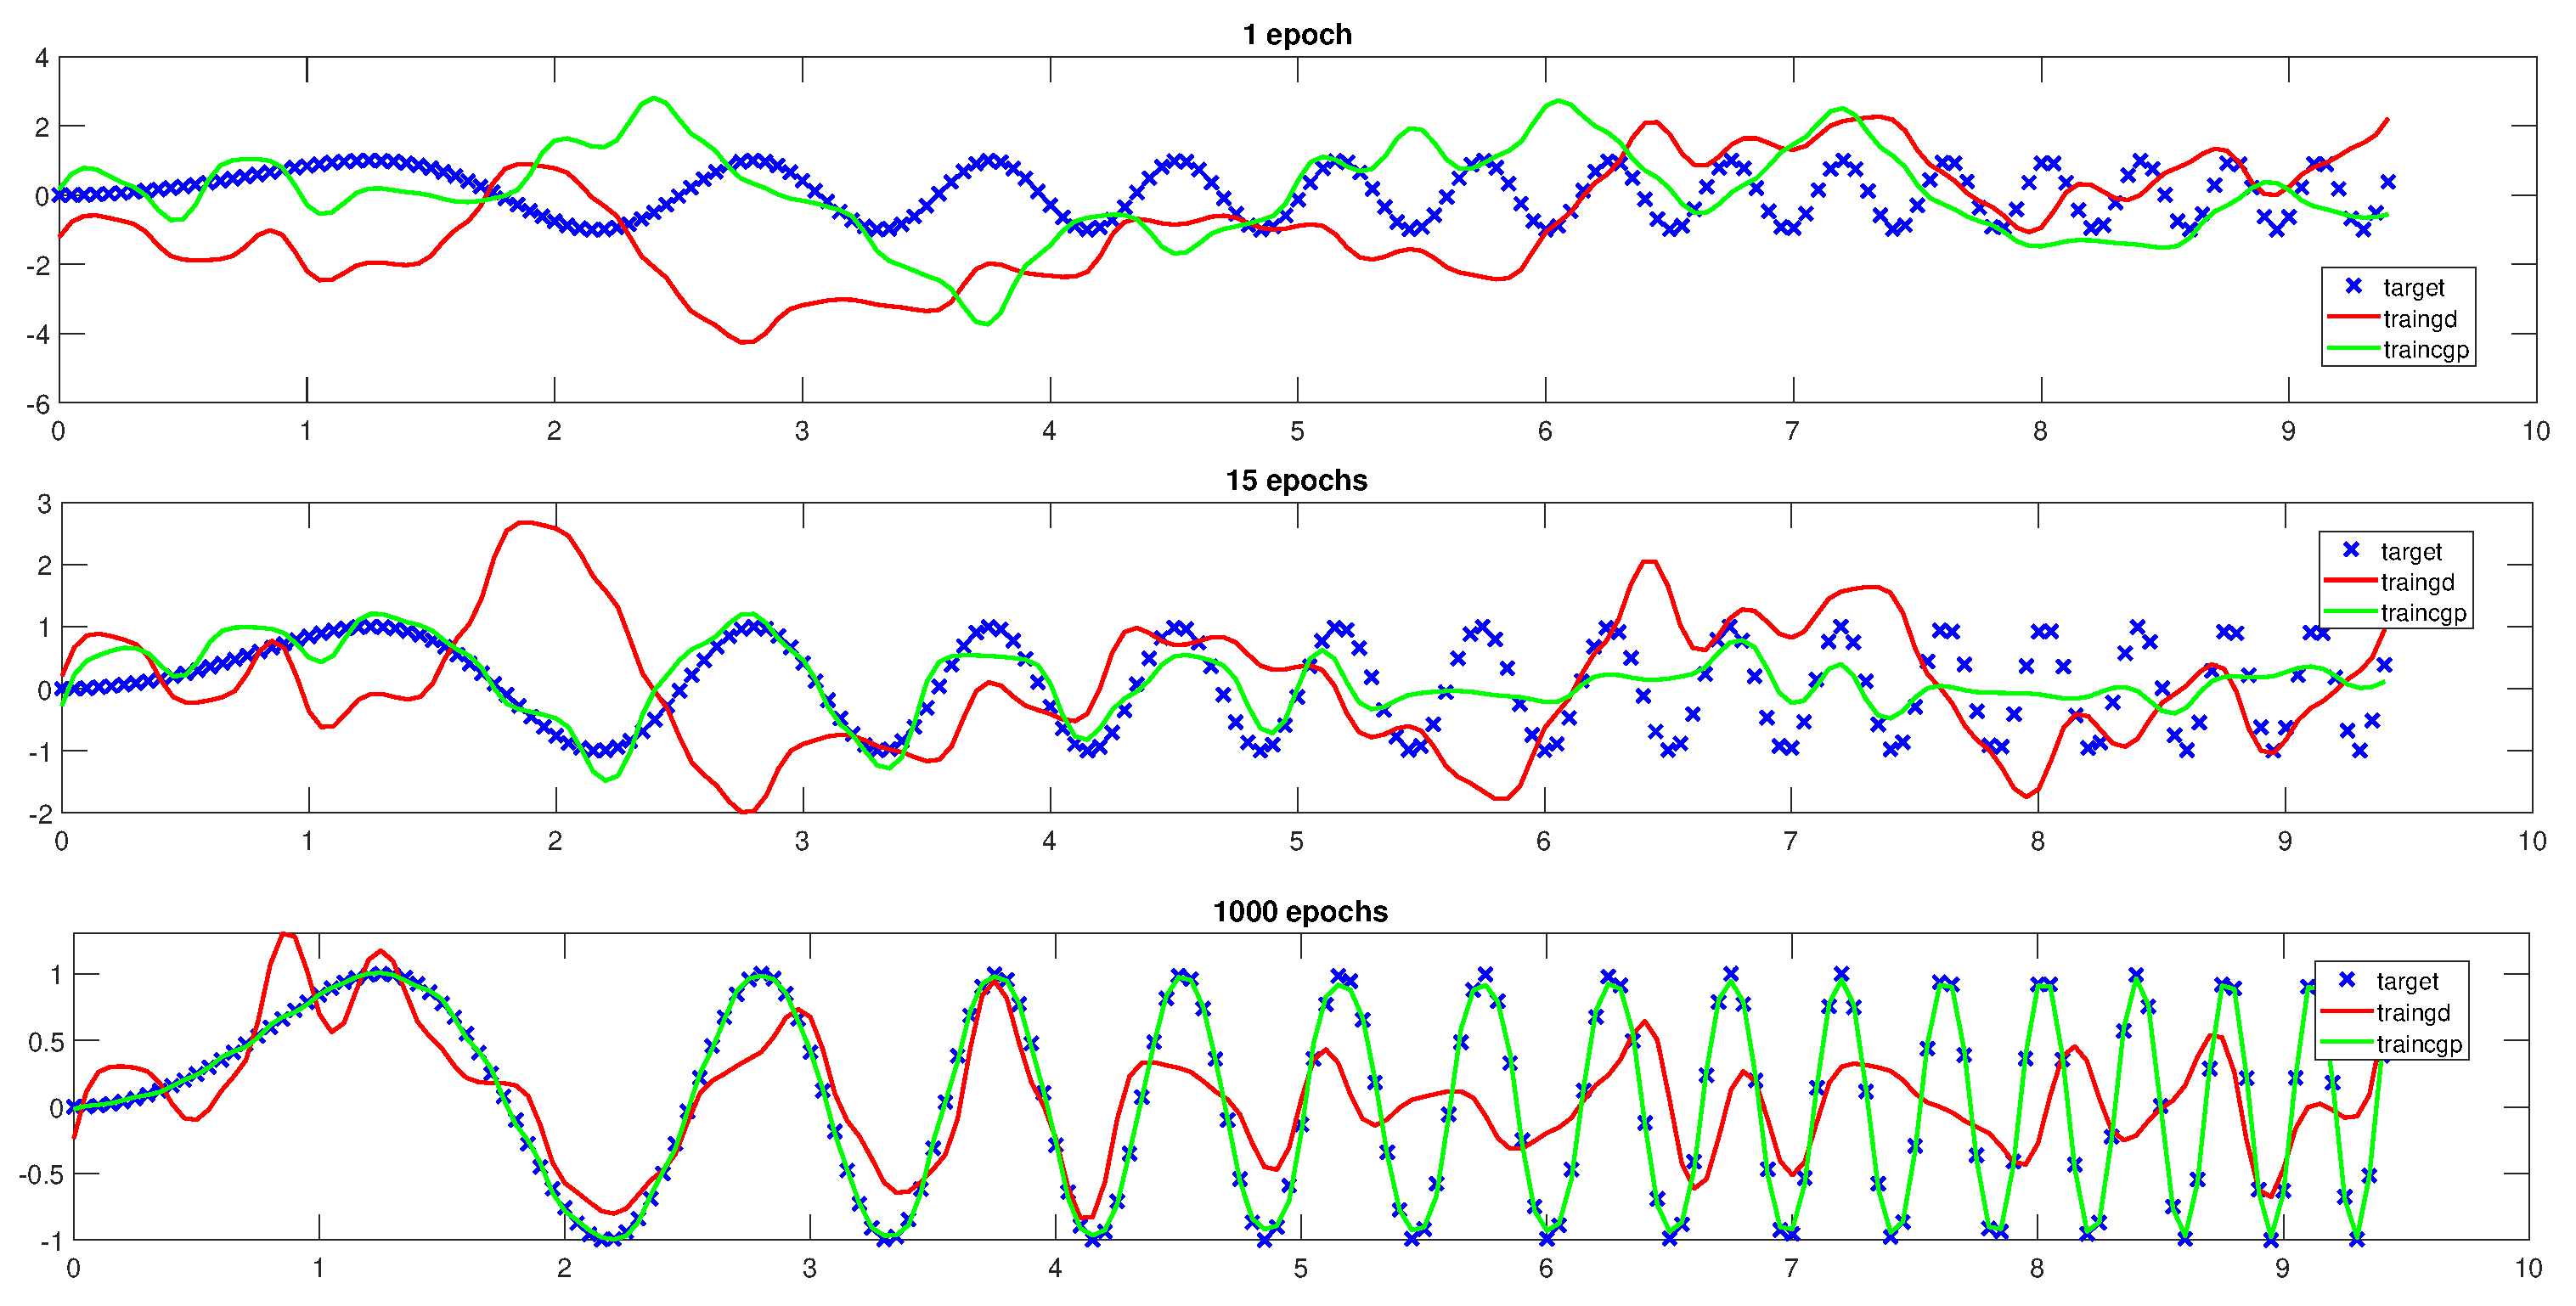
\includegraphics[height = 0.7\textwidth,width = 1\textwidth]{Exercise1/Report/train_gd_cgp}
		\caption{train\_gd VS  train\_cgp}\label{fig:train_gd_cgp}
	\end{subfigure}
	\begin{subfigure}[b]{0.33\textwidth}
		\centering
		\captionsetup{width=0.8\linewidth, format = hang}
		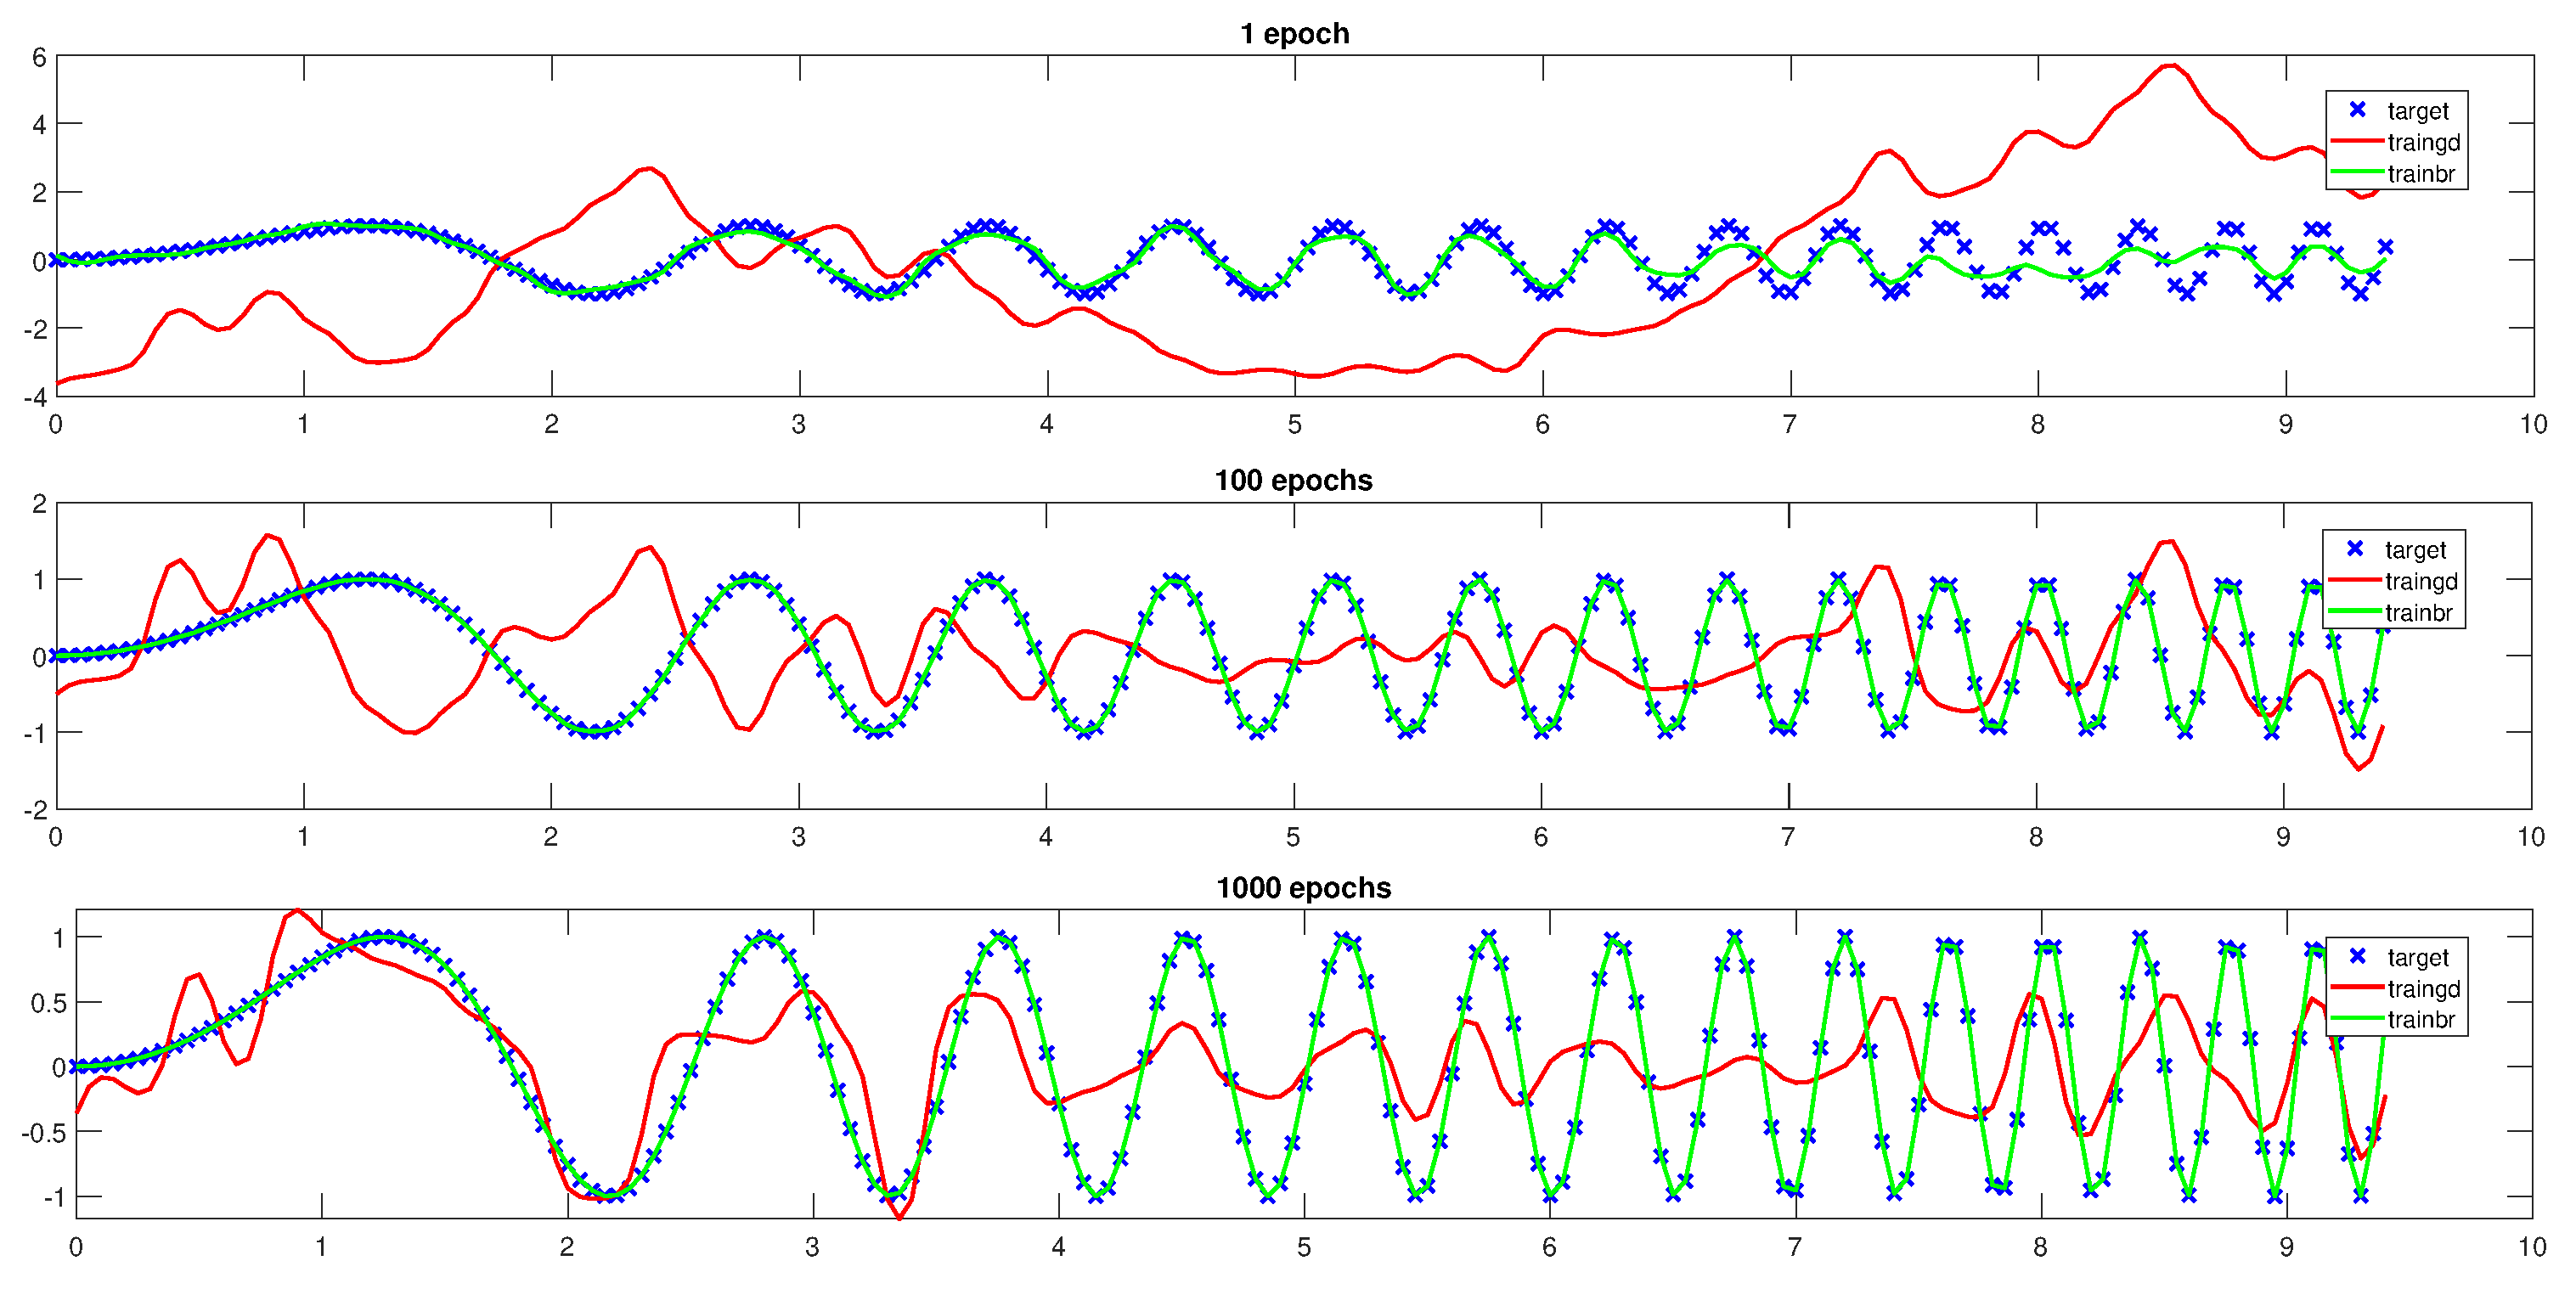
\includegraphics[height = 0.7\textwidth,width = 1\textwidth]{Exercise1/Report/train_gd_br}
		\caption{train\_gd VS  train\_br}\label{fig:train_gd_br)}
	\end{subfigure}%
	\begin{subfigure}[b]{0.33\textwidth}
		\centering
		\captionsetup{width=0.8\linewidth, format = hang}
		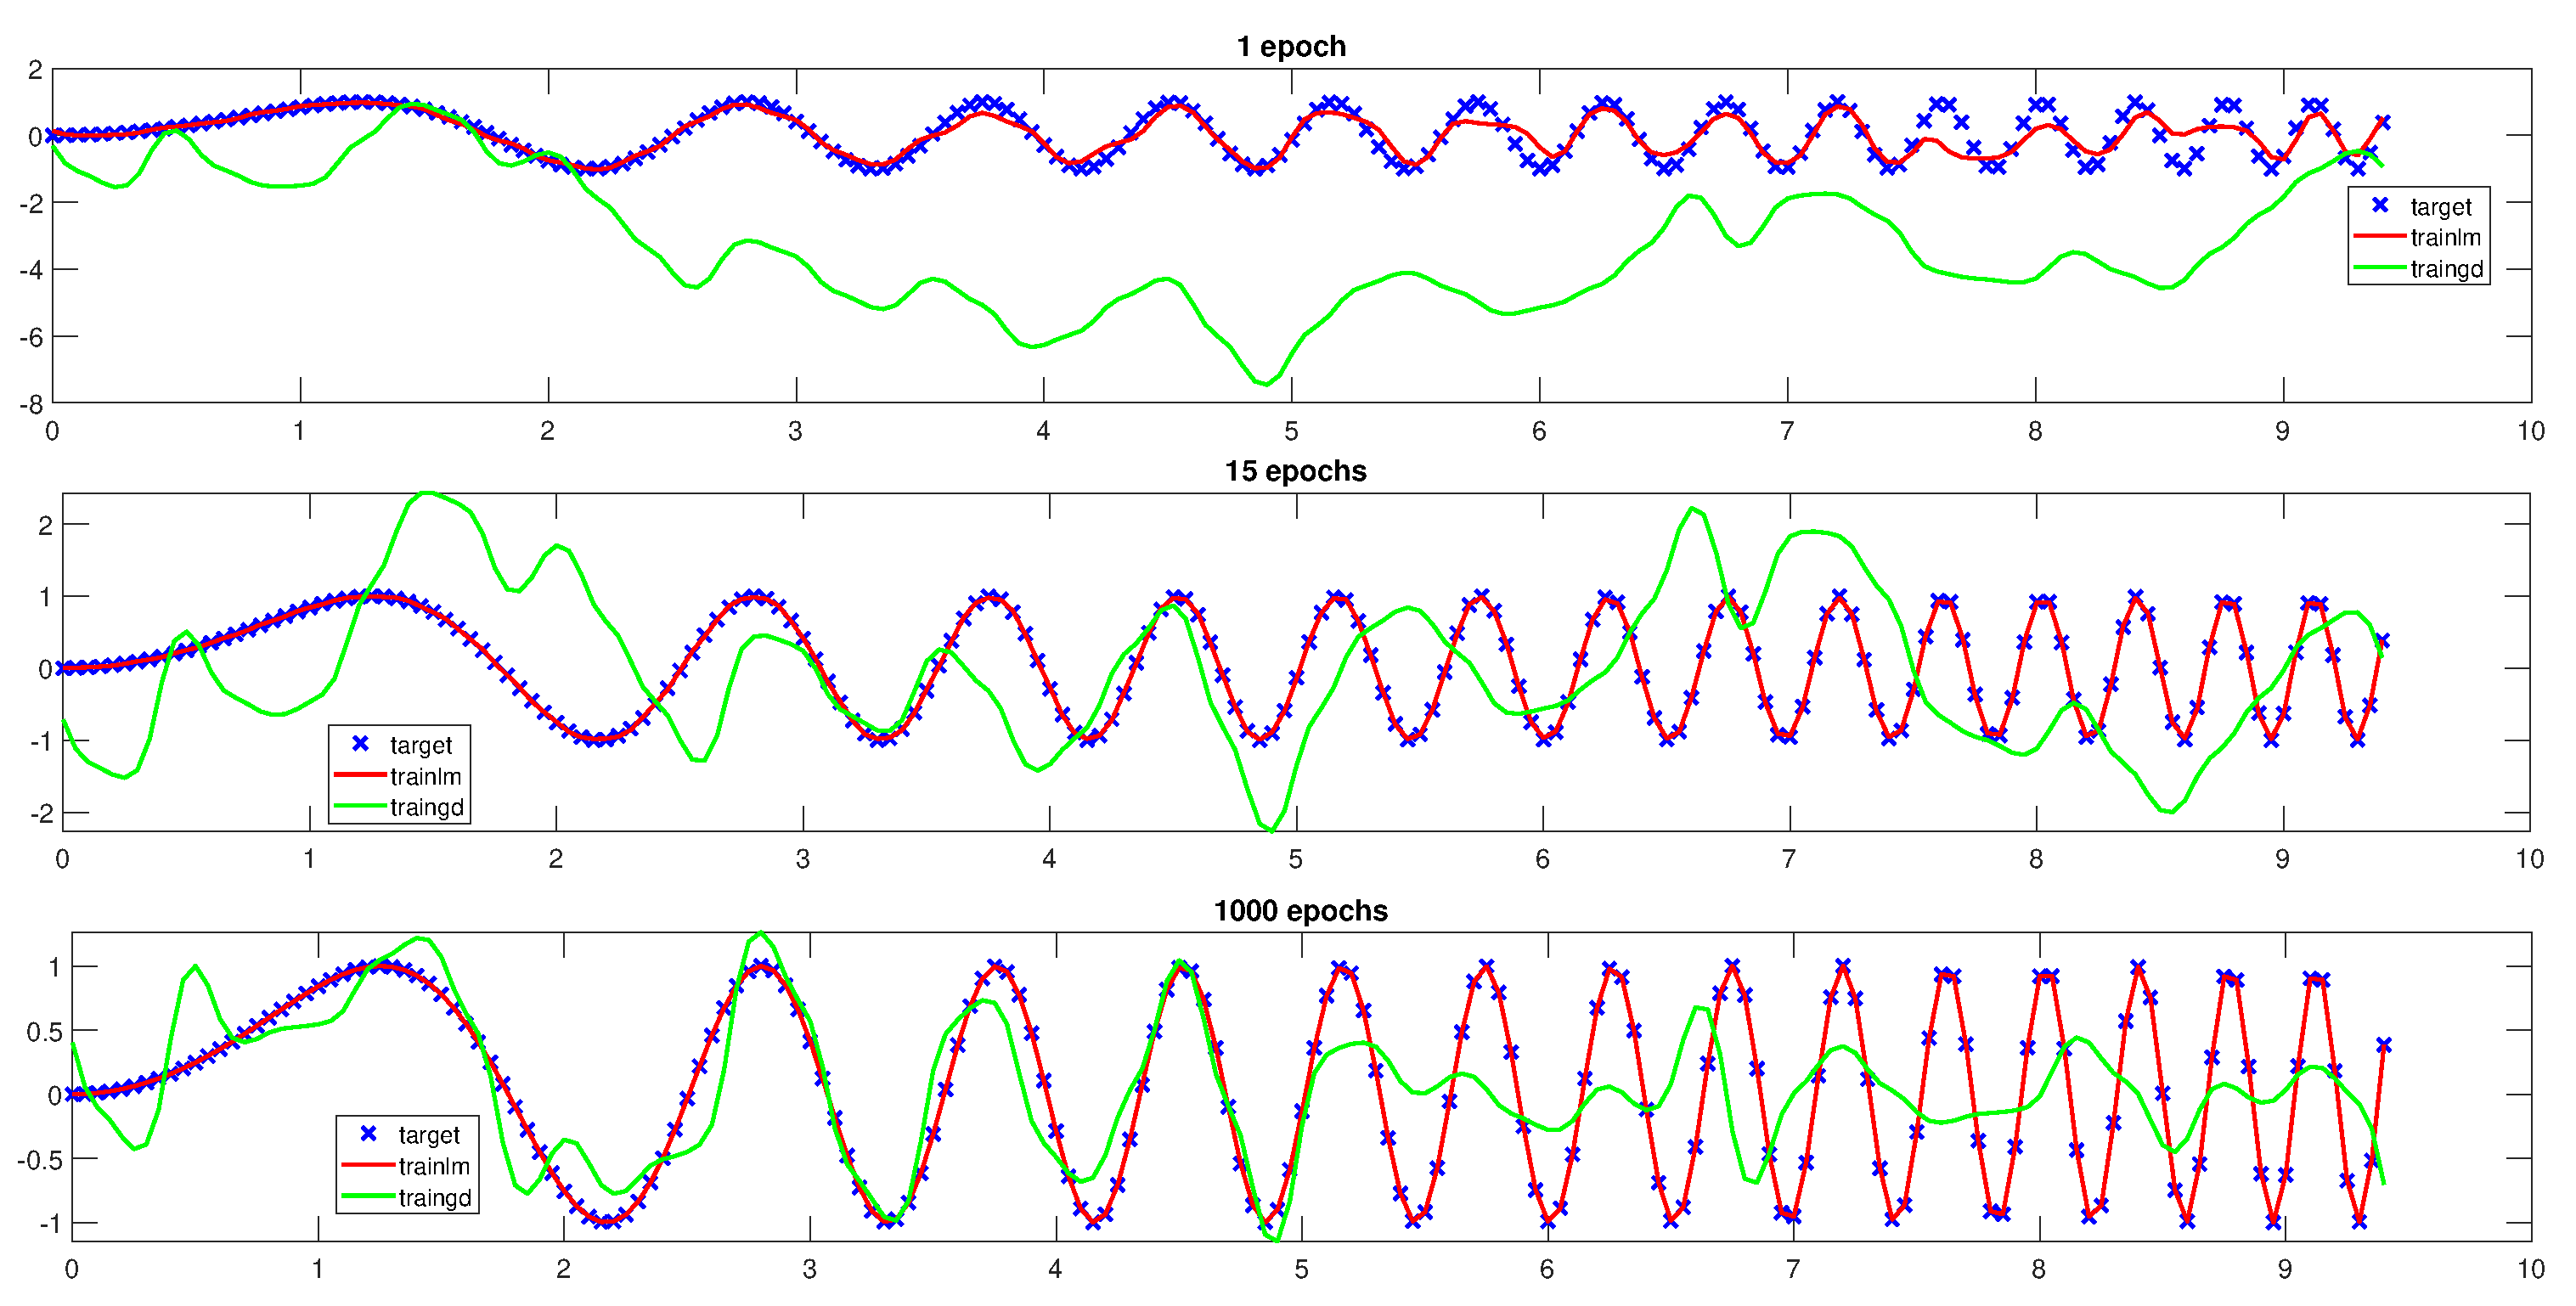
\includegraphics[height = 0.7\textwidth,width = 1\textwidth]{Exercise1/Report/train_lm_gd}
		\caption{train\_gd VS  train\_lm}\label{fig:train_lm_gd)}
	\end{subfigure}%
	\begin{subfigure}[b]{0.33\textwidth}
		\centering
		\captionsetup{width=0.8\linewidth, format = hang}
		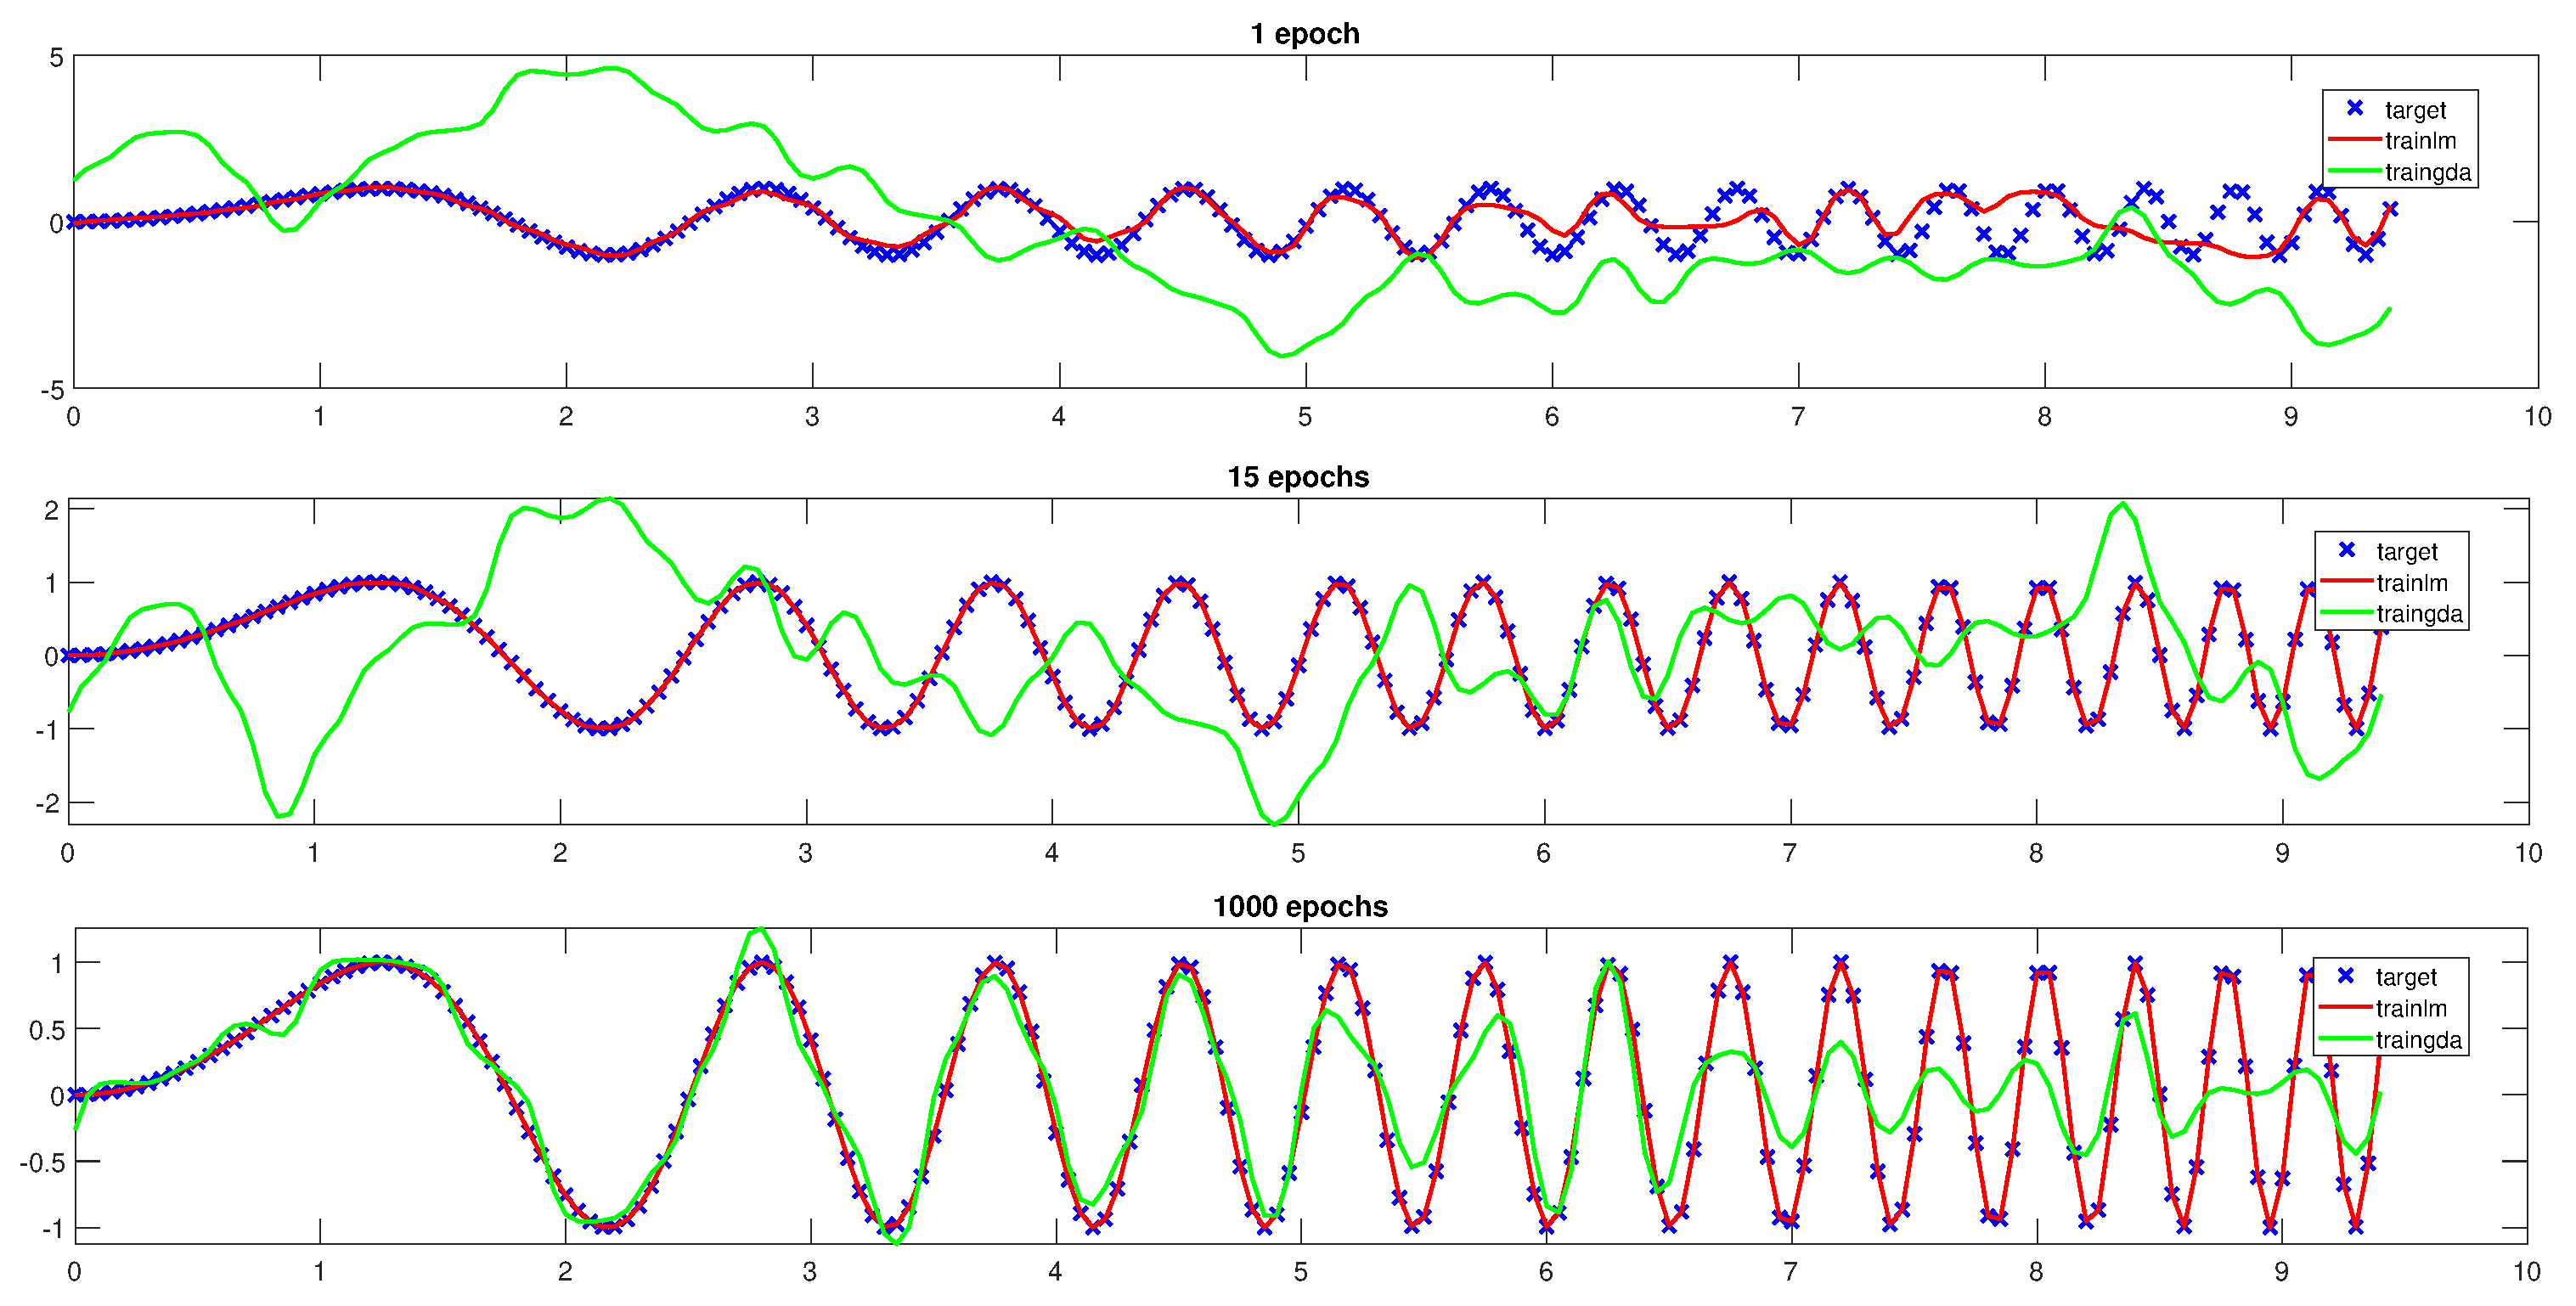
\includegraphics[height = 0.7\textwidth,width = 1\textwidth]{Exercise1/Report/train_lm_gda}
		\caption{train\_gda VS  train\_lm}\label{fig:train_lm_gda)}
	\end{subfigure}%
	\captionsetup{format = hang}
	\caption{Comparison of various training algorithm with gradient descent on input data without noise for [1;100;1000] epochs}
	\label{fig:train_gd}
\end{figure}

It can be seen from the figure that gradient descent performs the least amongst the other training algorithms. Gradient descent with adaptive learning rate performs better than the normal gradient descent. The function approximations is done by reducing the mean square errors over the training epoch. If the number of epochs is increased then gradient descent also gives better approximations just like other algorithms as shown in the figure \ref{fig:train_lm_gd_2}.
\begin{figure}
	\begin{subfigure}[b]{0.33\textwidth}
 		\centering
 		\captionsetup{width=1\linewidth, format = hang}
 		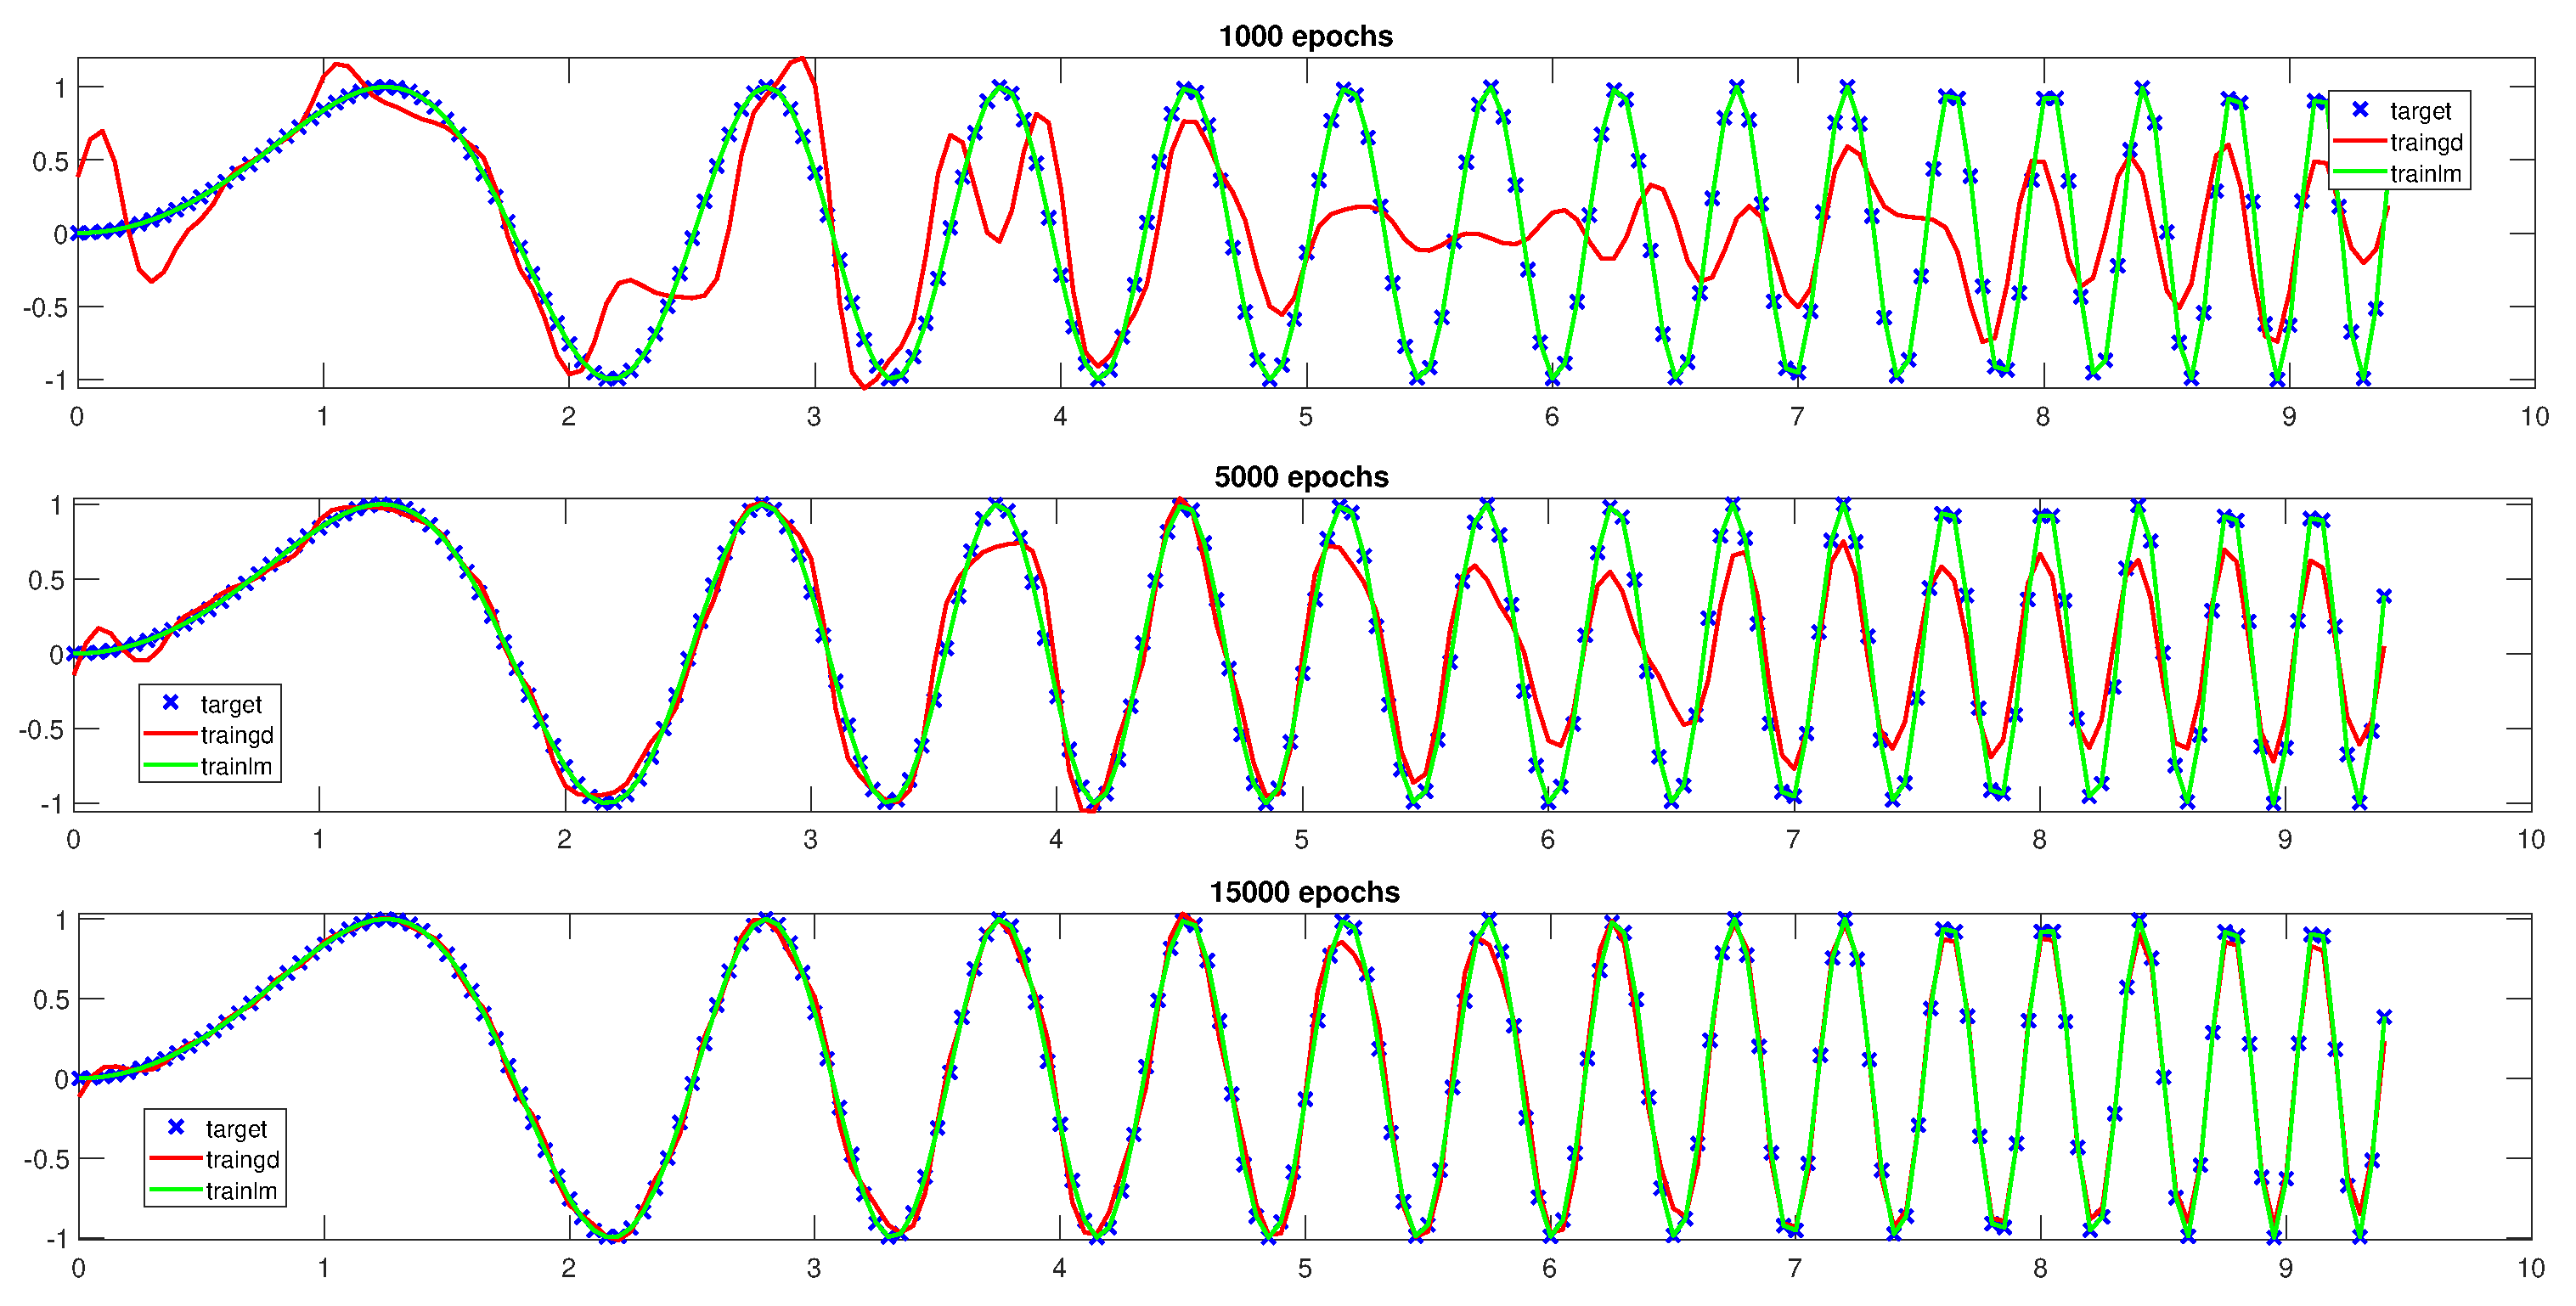
\includegraphics[height = 0.7\textwidth,width = 1\textwidth]{Exercise1/Report/train_lm_gd_2}
	 	\caption{train\_lm VS  train\_gd for epochs [1000;5000;15000]}\label{fig:train_lm_gd_2}
	 \end{subfigure}%
	 \begin{subfigure}[b]{0.33\textwidth}
 		\centering
 		\captionsetup{width=0.8\linewidth, format = hang}
 		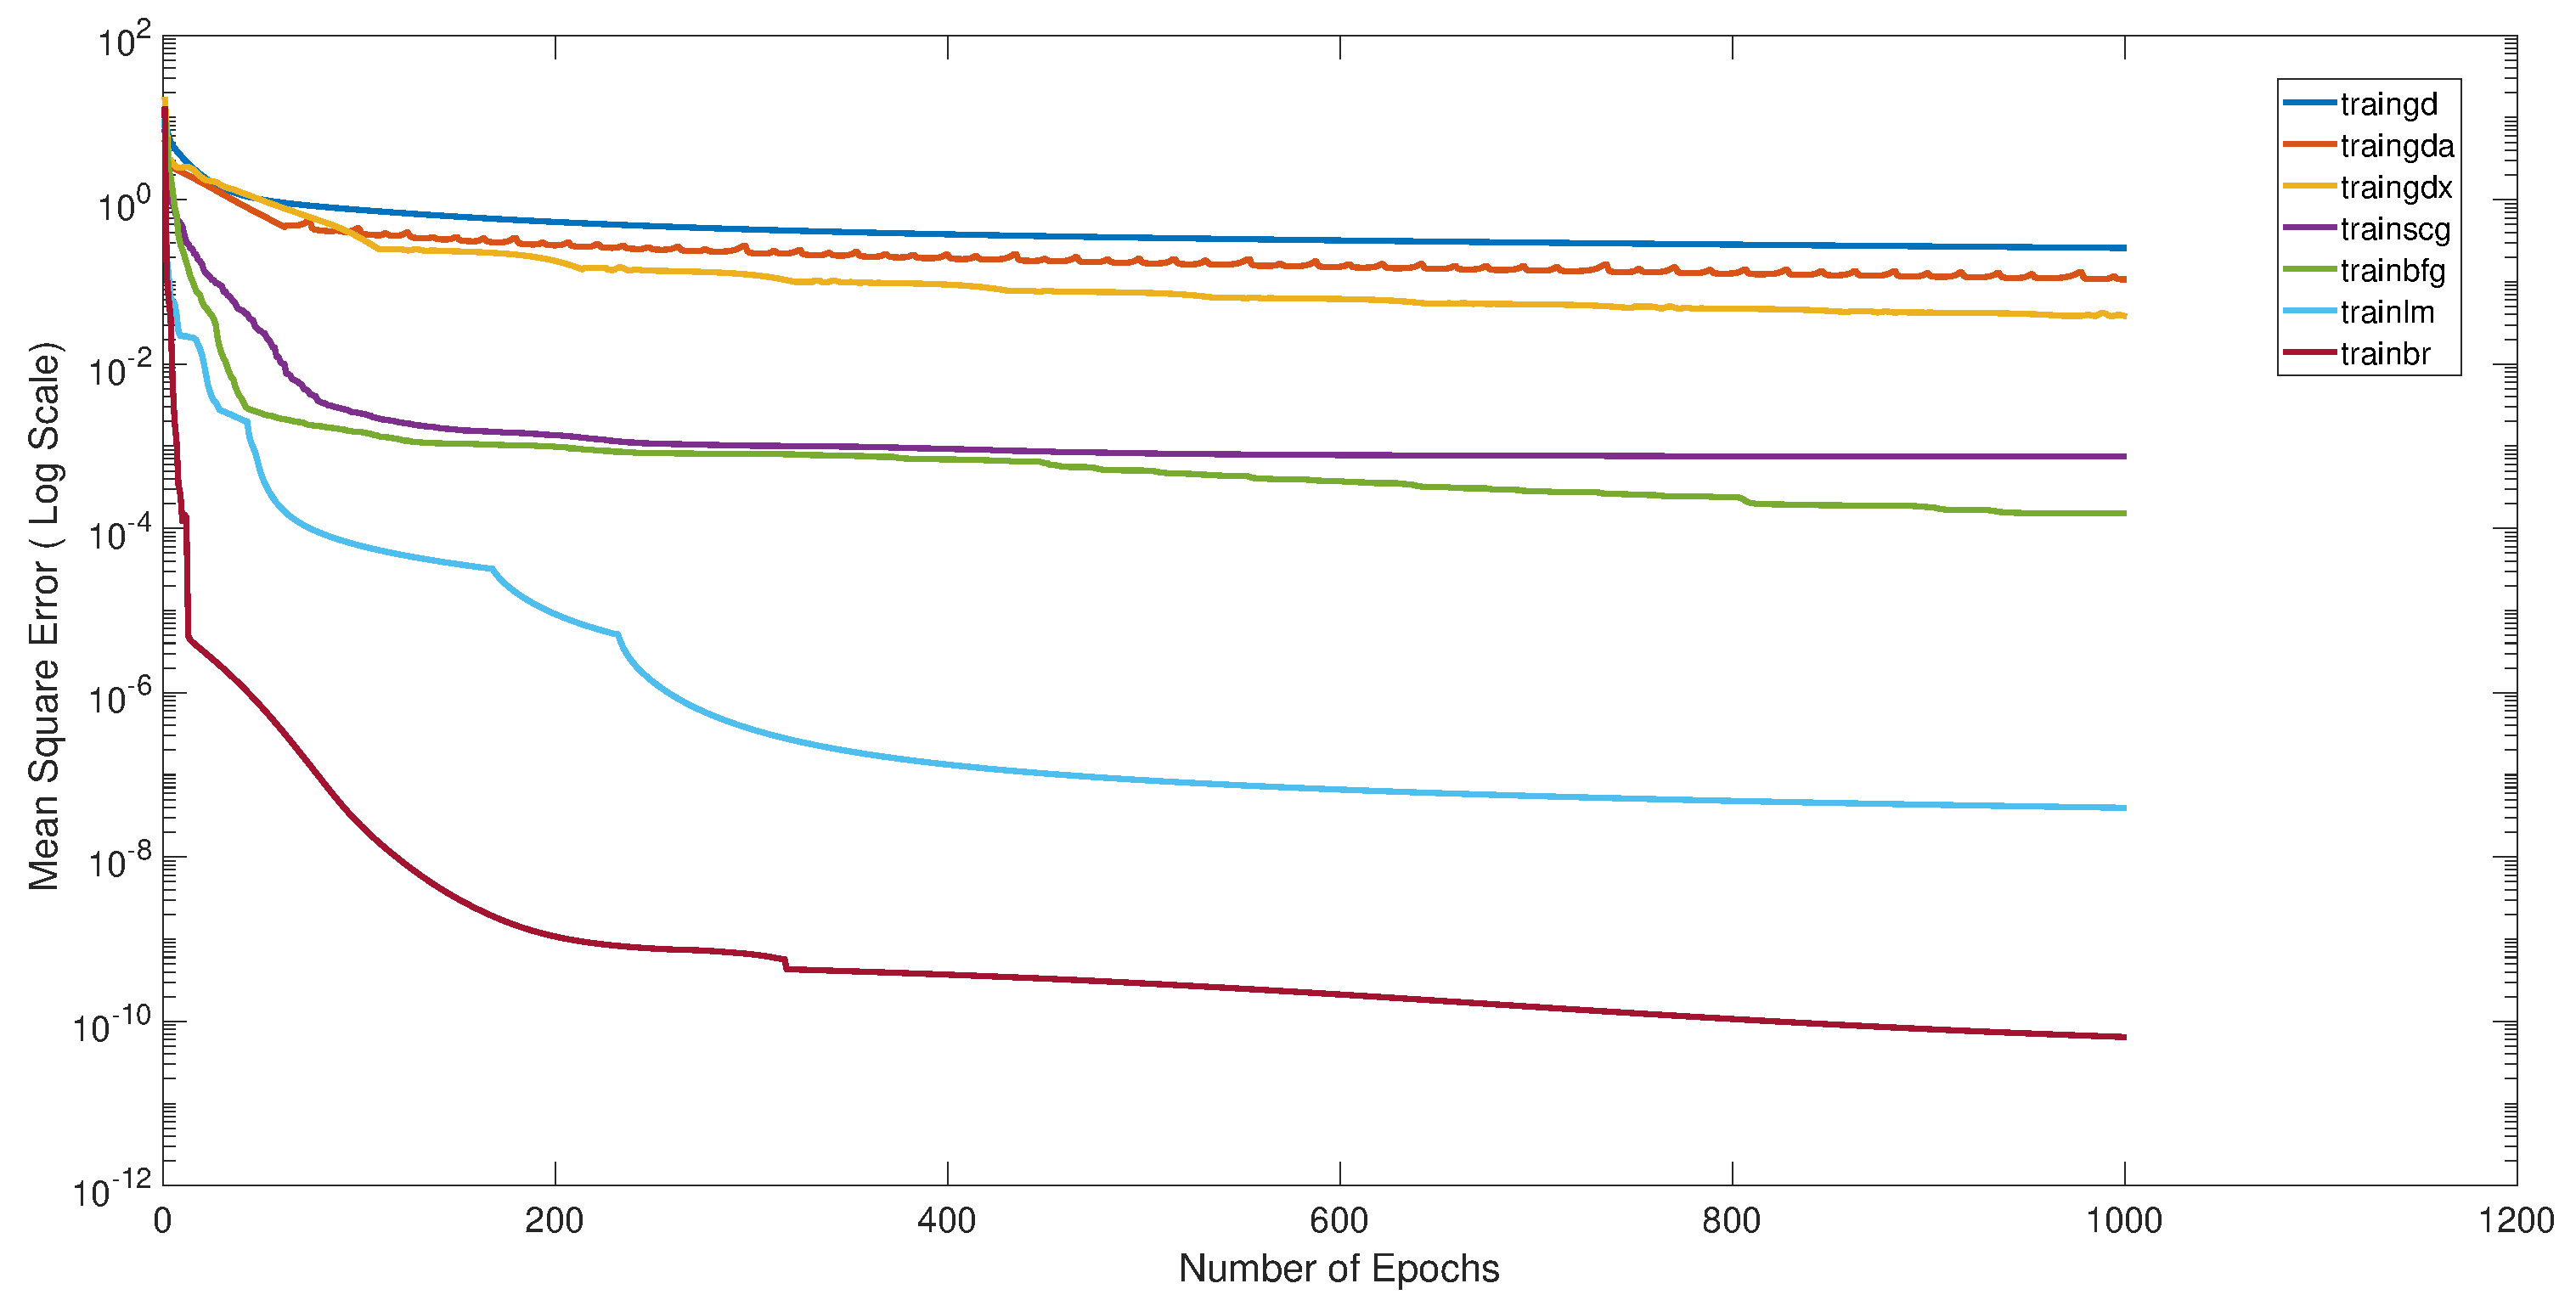
\includegraphics[height = 0.7\textwidth,width = 1\textwidth]{Exercise1/Report/mse_1}
 		\caption{MSE VS Number of training epochs}\label{fig:mse_1}
 	\end{subfigure}%
	 \begin{subfigure}[b]{0.33\textwidth}
 		\centering
 		\captionsetup{width=0.8\linewidth, format = hang}
 		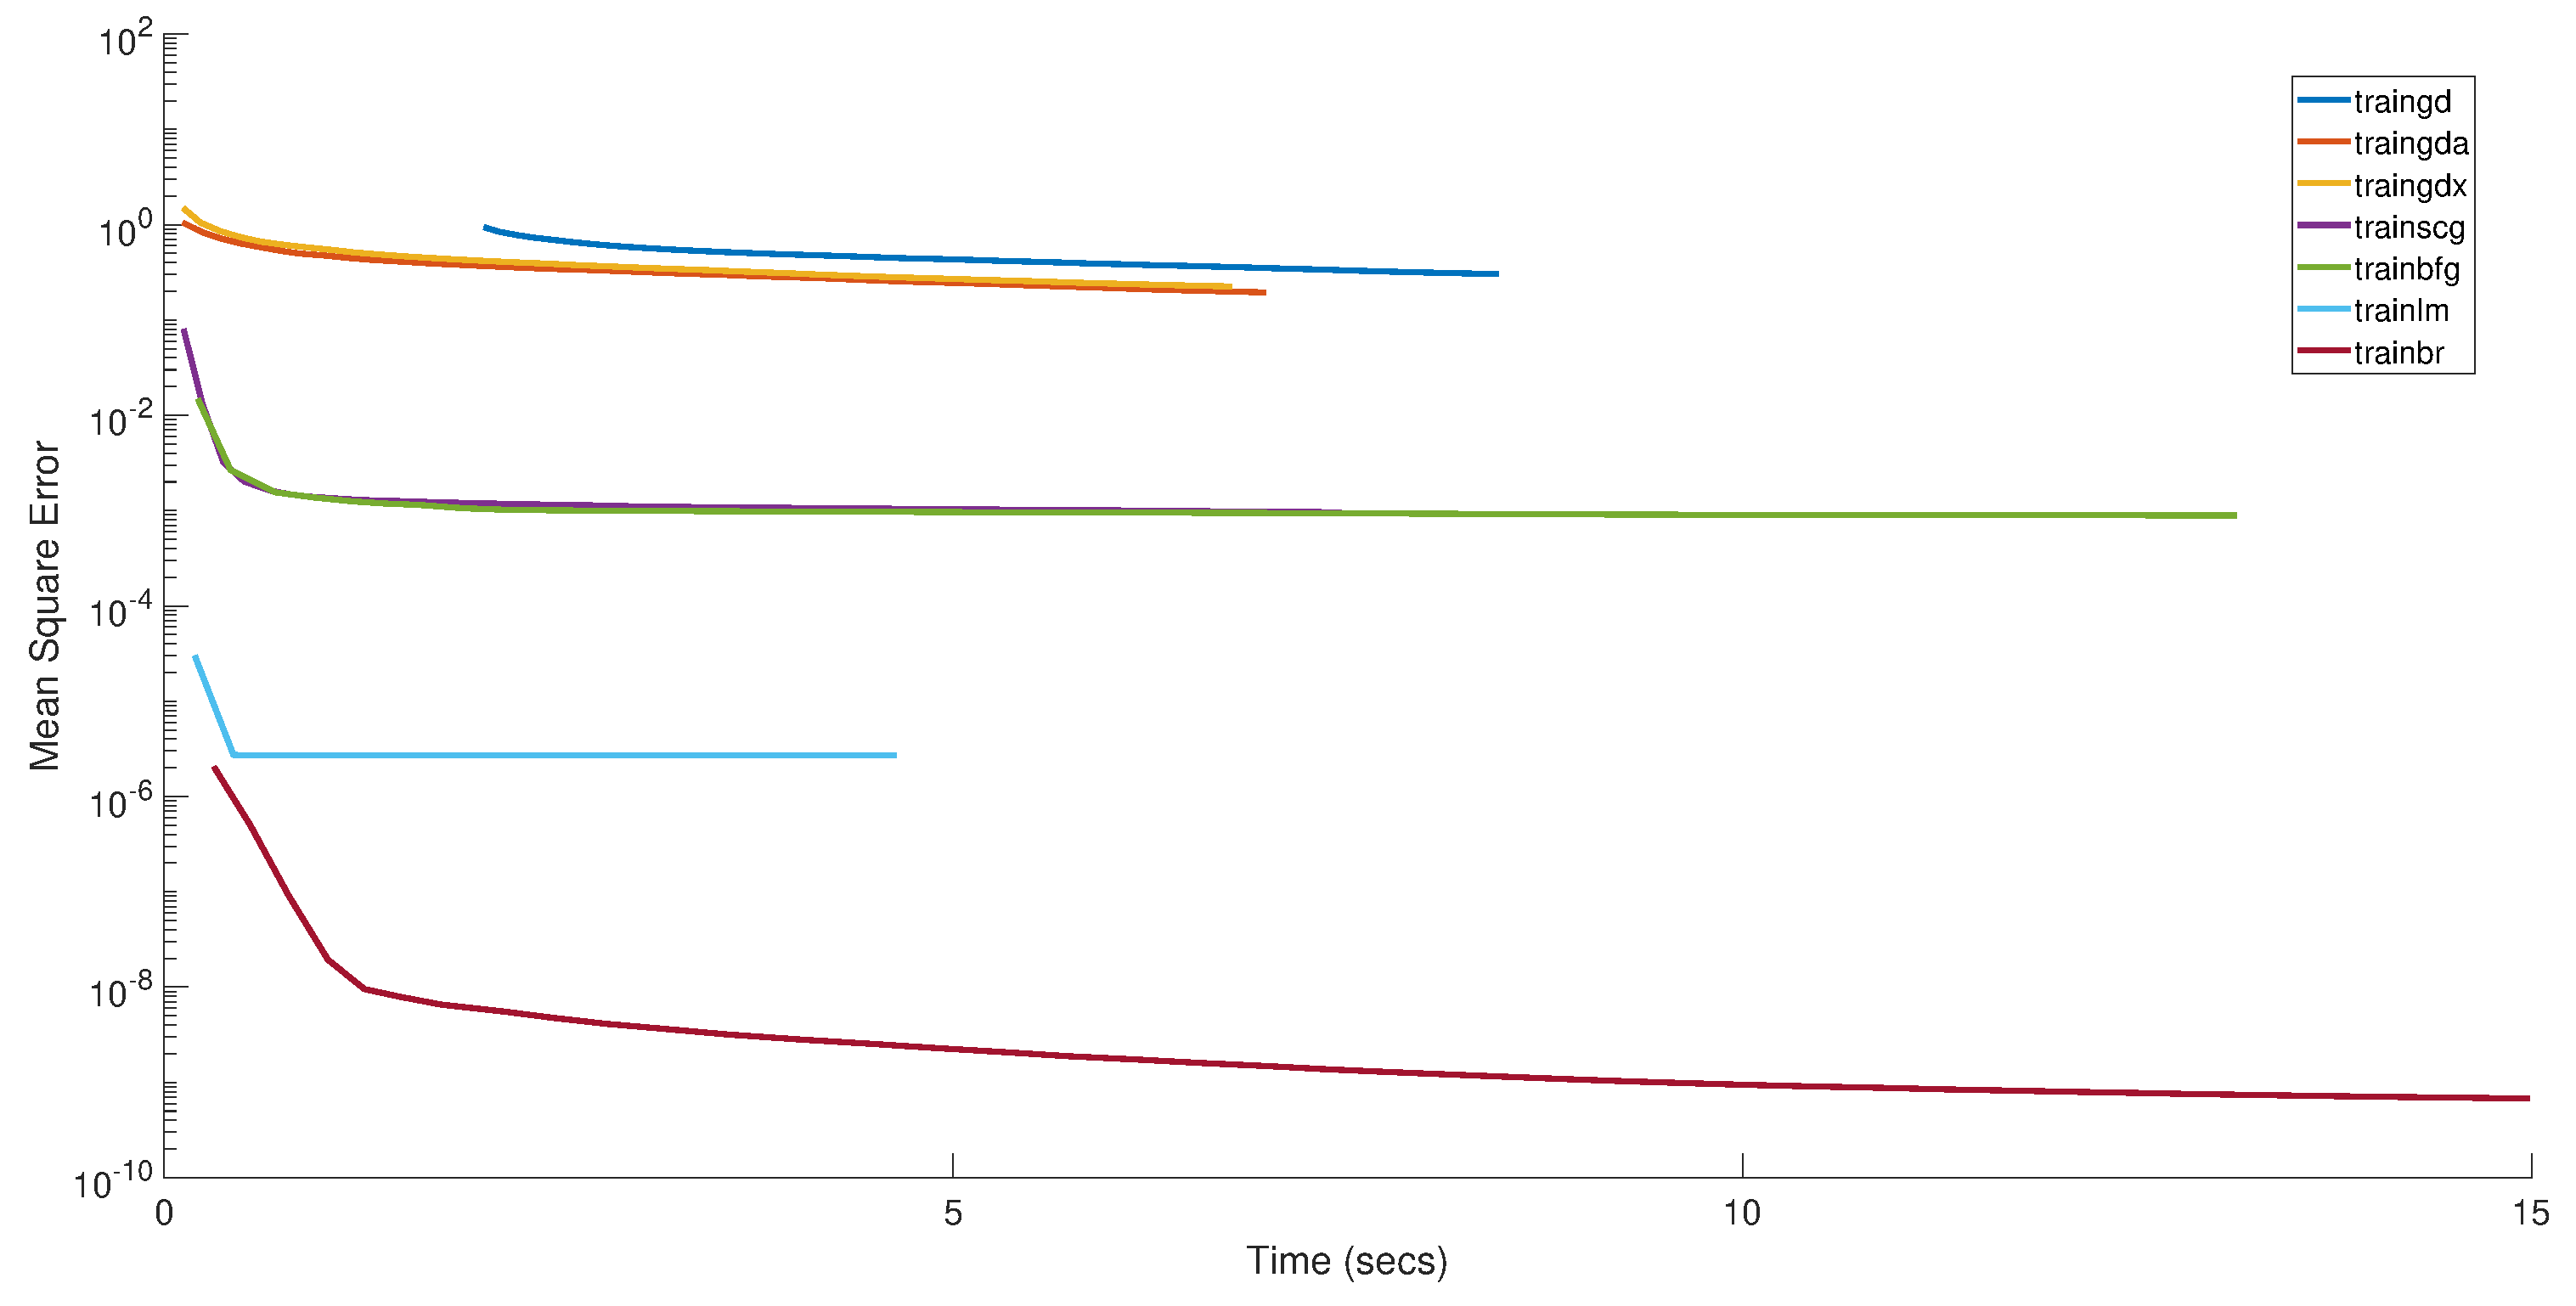
\includegraphics[height = 0.7\textwidth,width = 1\textwidth]{Exercise1/Report/mse_2}
 		\caption{MSE VS Training time \newline}\label{fig:mse_2}
 	\end{subfigure}
 	\captionsetup{format = hang}
 	\caption{Performance of various training algorithms on input data without noise}
 	\label{fig:train_perf}
\end{figure}
From figures \ref{fig:mse_1} and \ref{fig:mse_2}, it can be seen that training algorithm with Levenberg-Marquardt with Bayesian regularization \textit{(trainbr)} has the least MSE but training time is slightly more. Overall Levenberg-Marquardt \textit{(trainlm)} is the best with minimum training time and mean square errors.  

Similar observations can be seen for the input data with noise added via $y=sin(x^2)+\sigma*randn(1,length(x))$, where $\sigma$ is noise level and chosen as 0.5. the performance of Levenberg-Marquardt is best on this noisy data. Also, gradient descent gives good approximation if the number of epochs is increased as shown in figure. This is because for larger iterations, the convergence rate increases.

\begin{figure}[!htpb]
	\begin{subfigure}[b]{0.33\textwidth}
		\centering
		\captionsetup{width=1\linewidth, format = hang}
		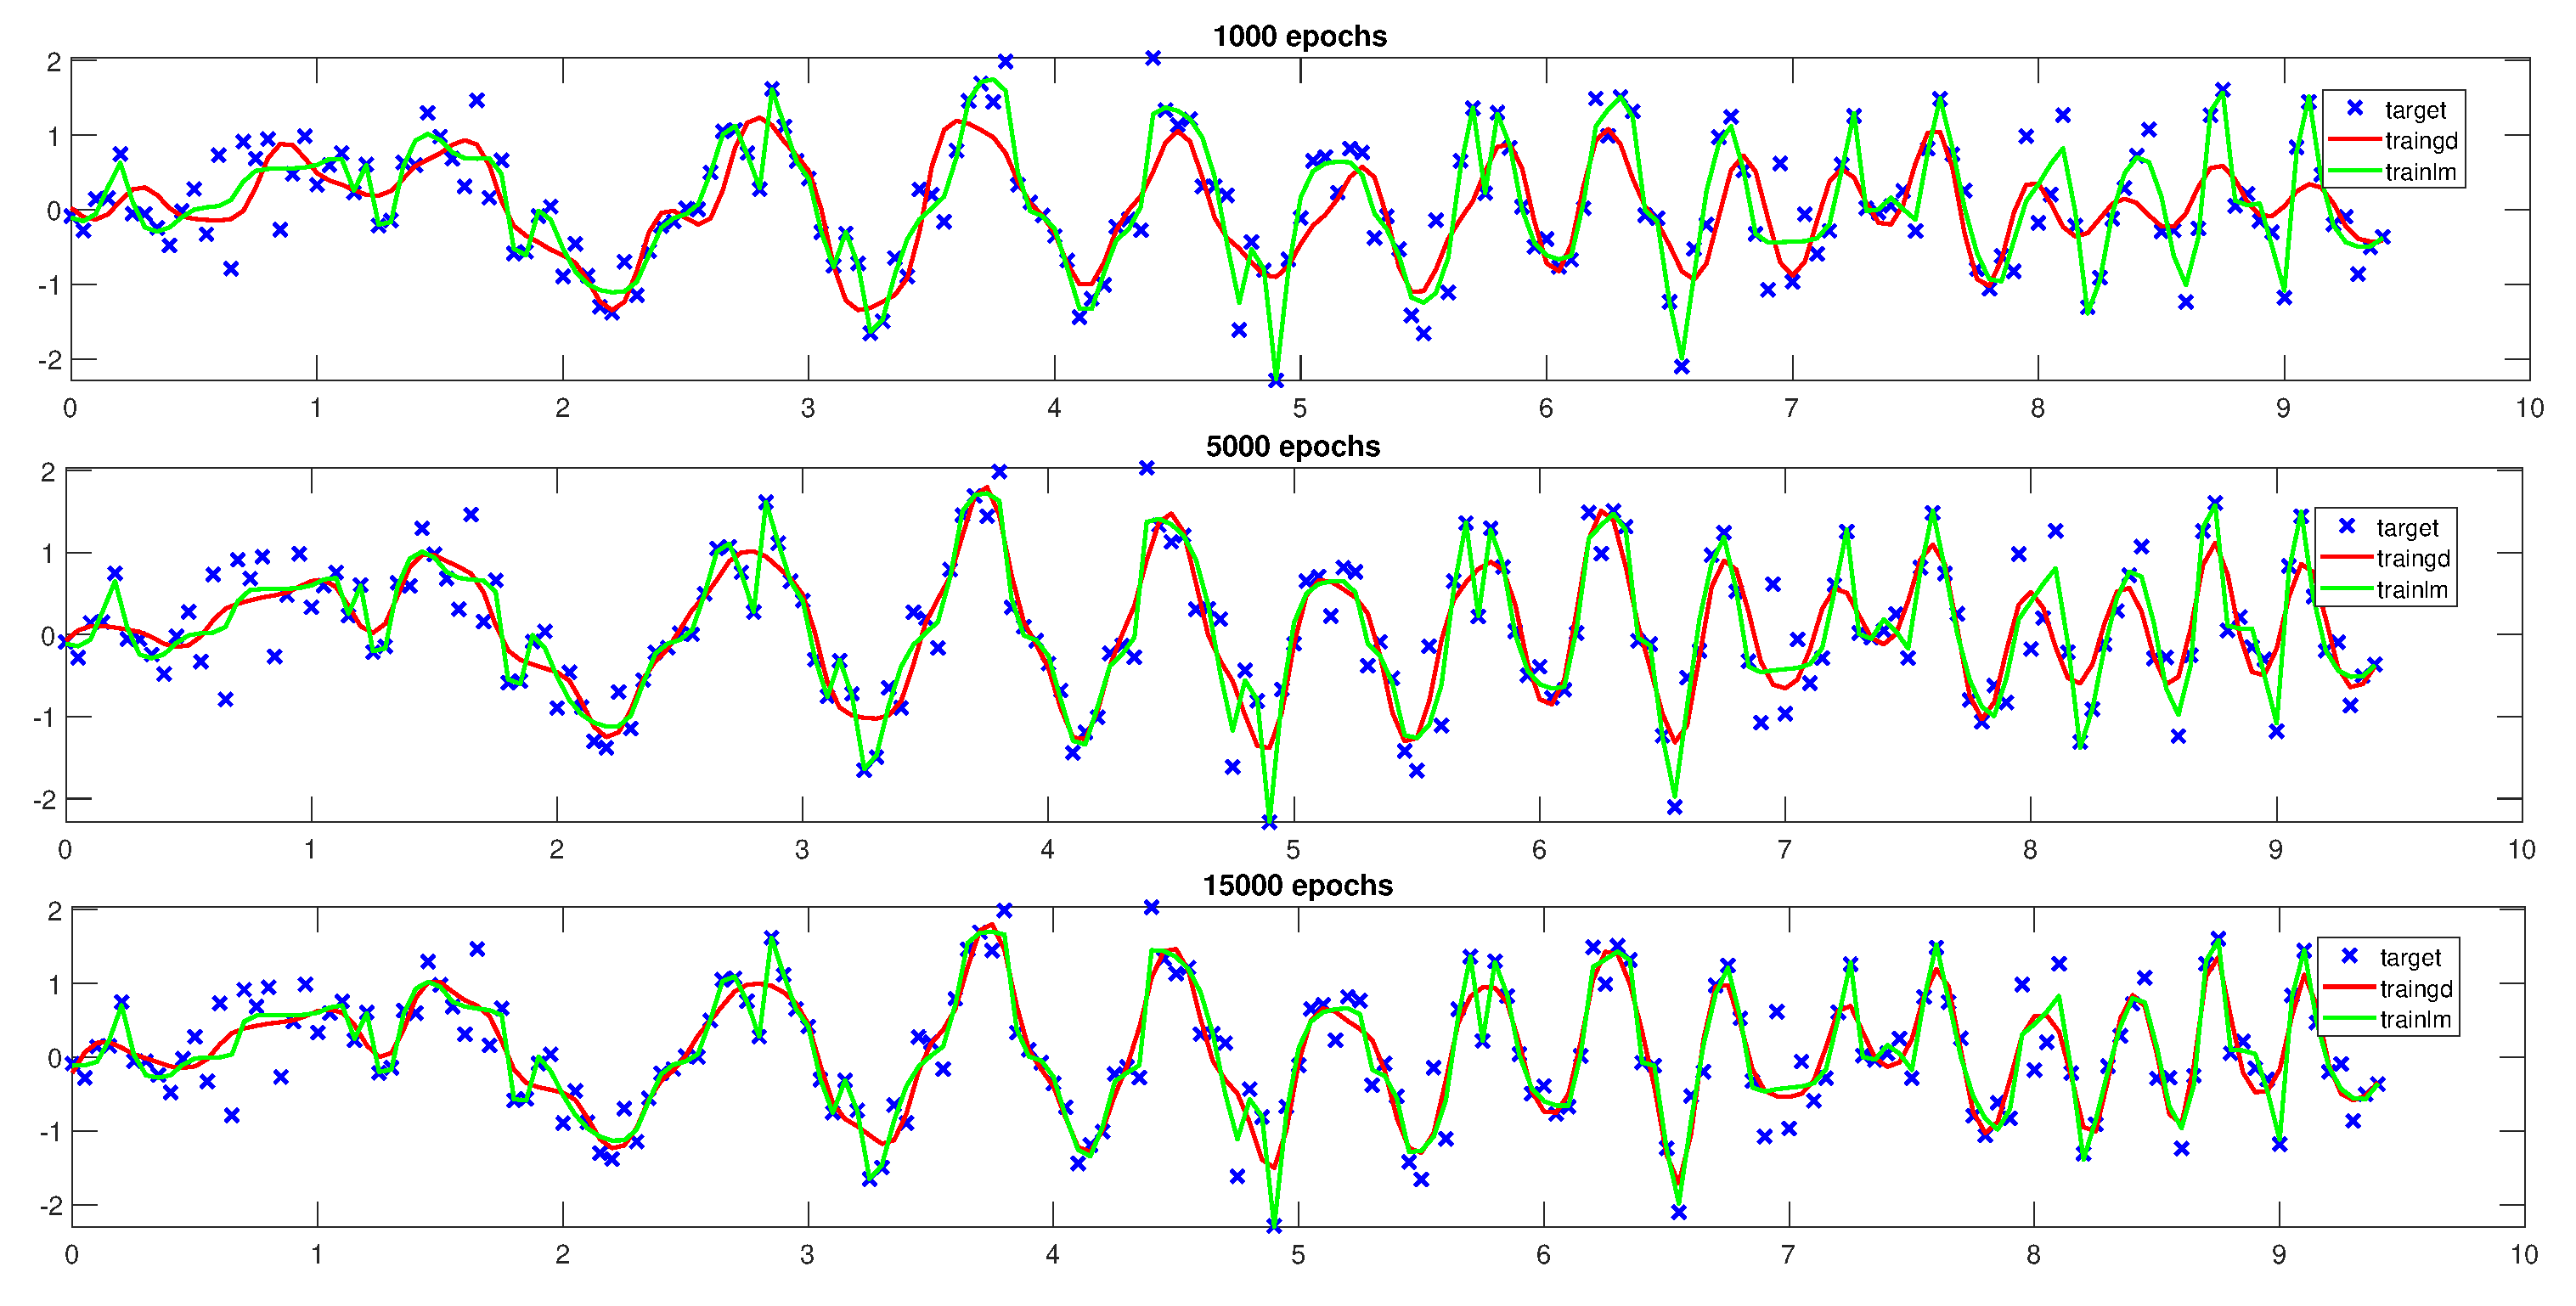
\includegraphics[height = 0.7\textwidth,width = 1\textwidth]{Exercise1/Report/train_lm_gd_noise_2}
		\caption{train\_lm VS  train\_gd for epochs [1000;5000;15000]}\label{fig:train_lm_gd_noise_2}
	\end{subfigure}%
	\begin{subfigure}[b]{0.33\textwidth}
		\centering
		\captionsetup{width=0.8\linewidth, format = hang}
		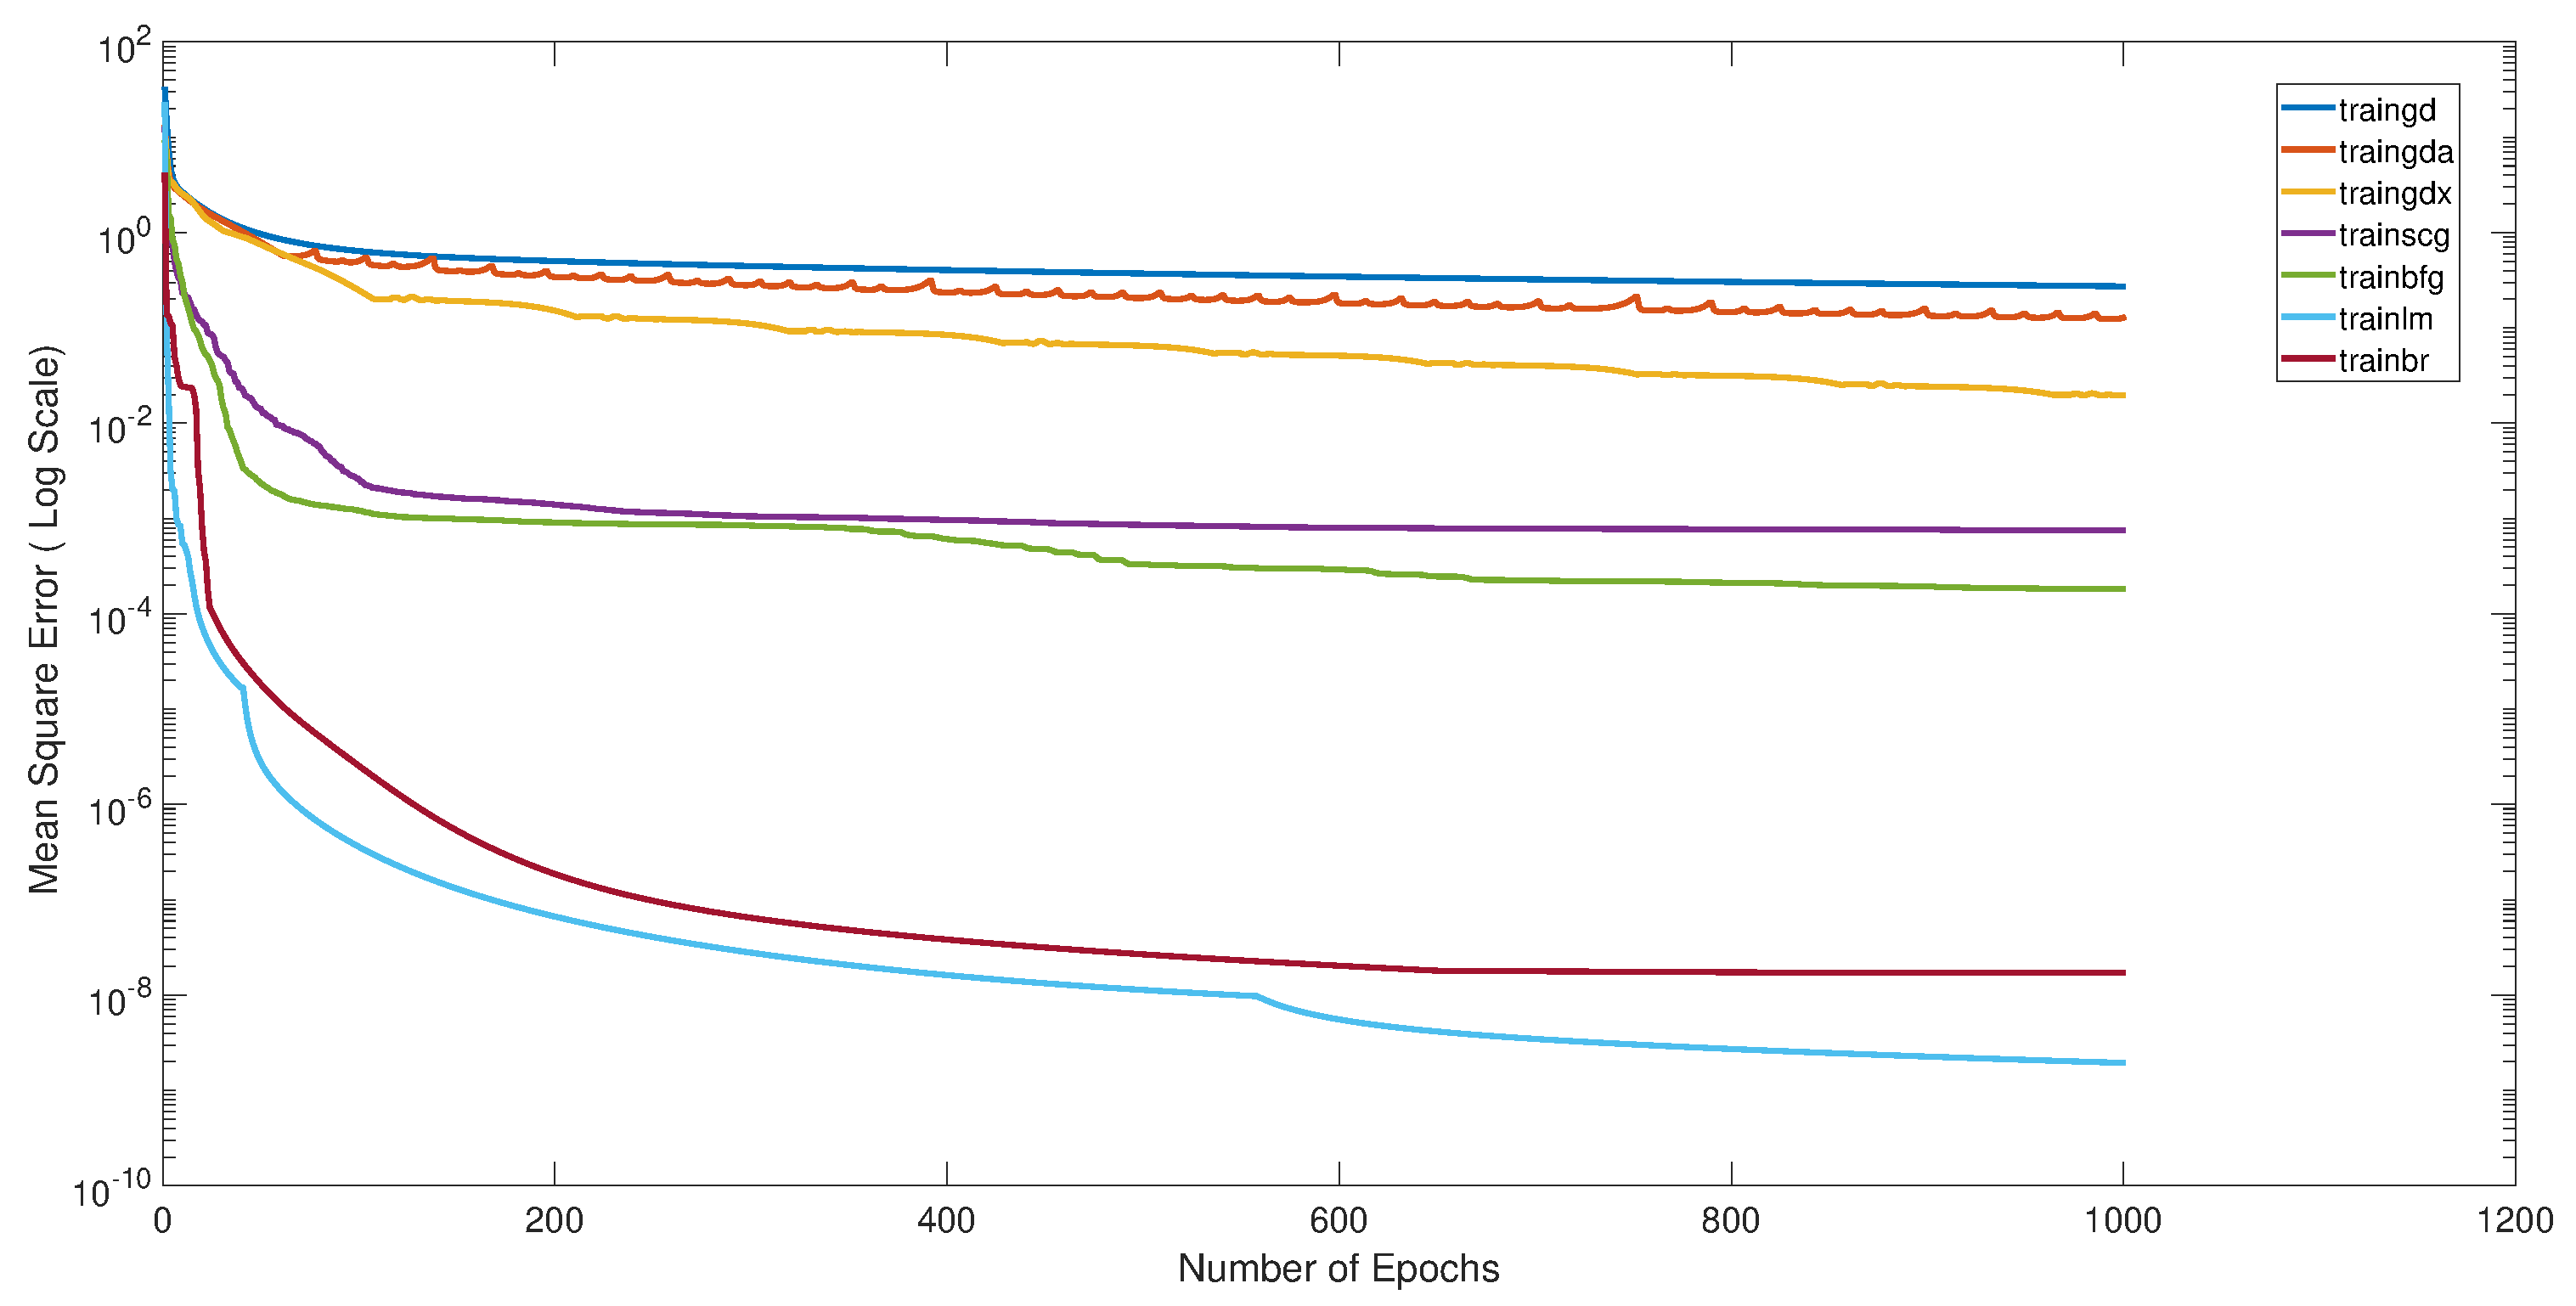
\includegraphics[height = 0.7\textwidth,width = 1\textwidth]{Exercise1/Report/mse_1_noise}
		\caption{MSE VS Number of training epochs}\label{fig:mse_1_noise}
	\end{subfigure}%
	\begin{subfigure}[b]{0.33\textwidth}
		\centering
		\captionsetup{width=0.8\linewidth, format = hang}
		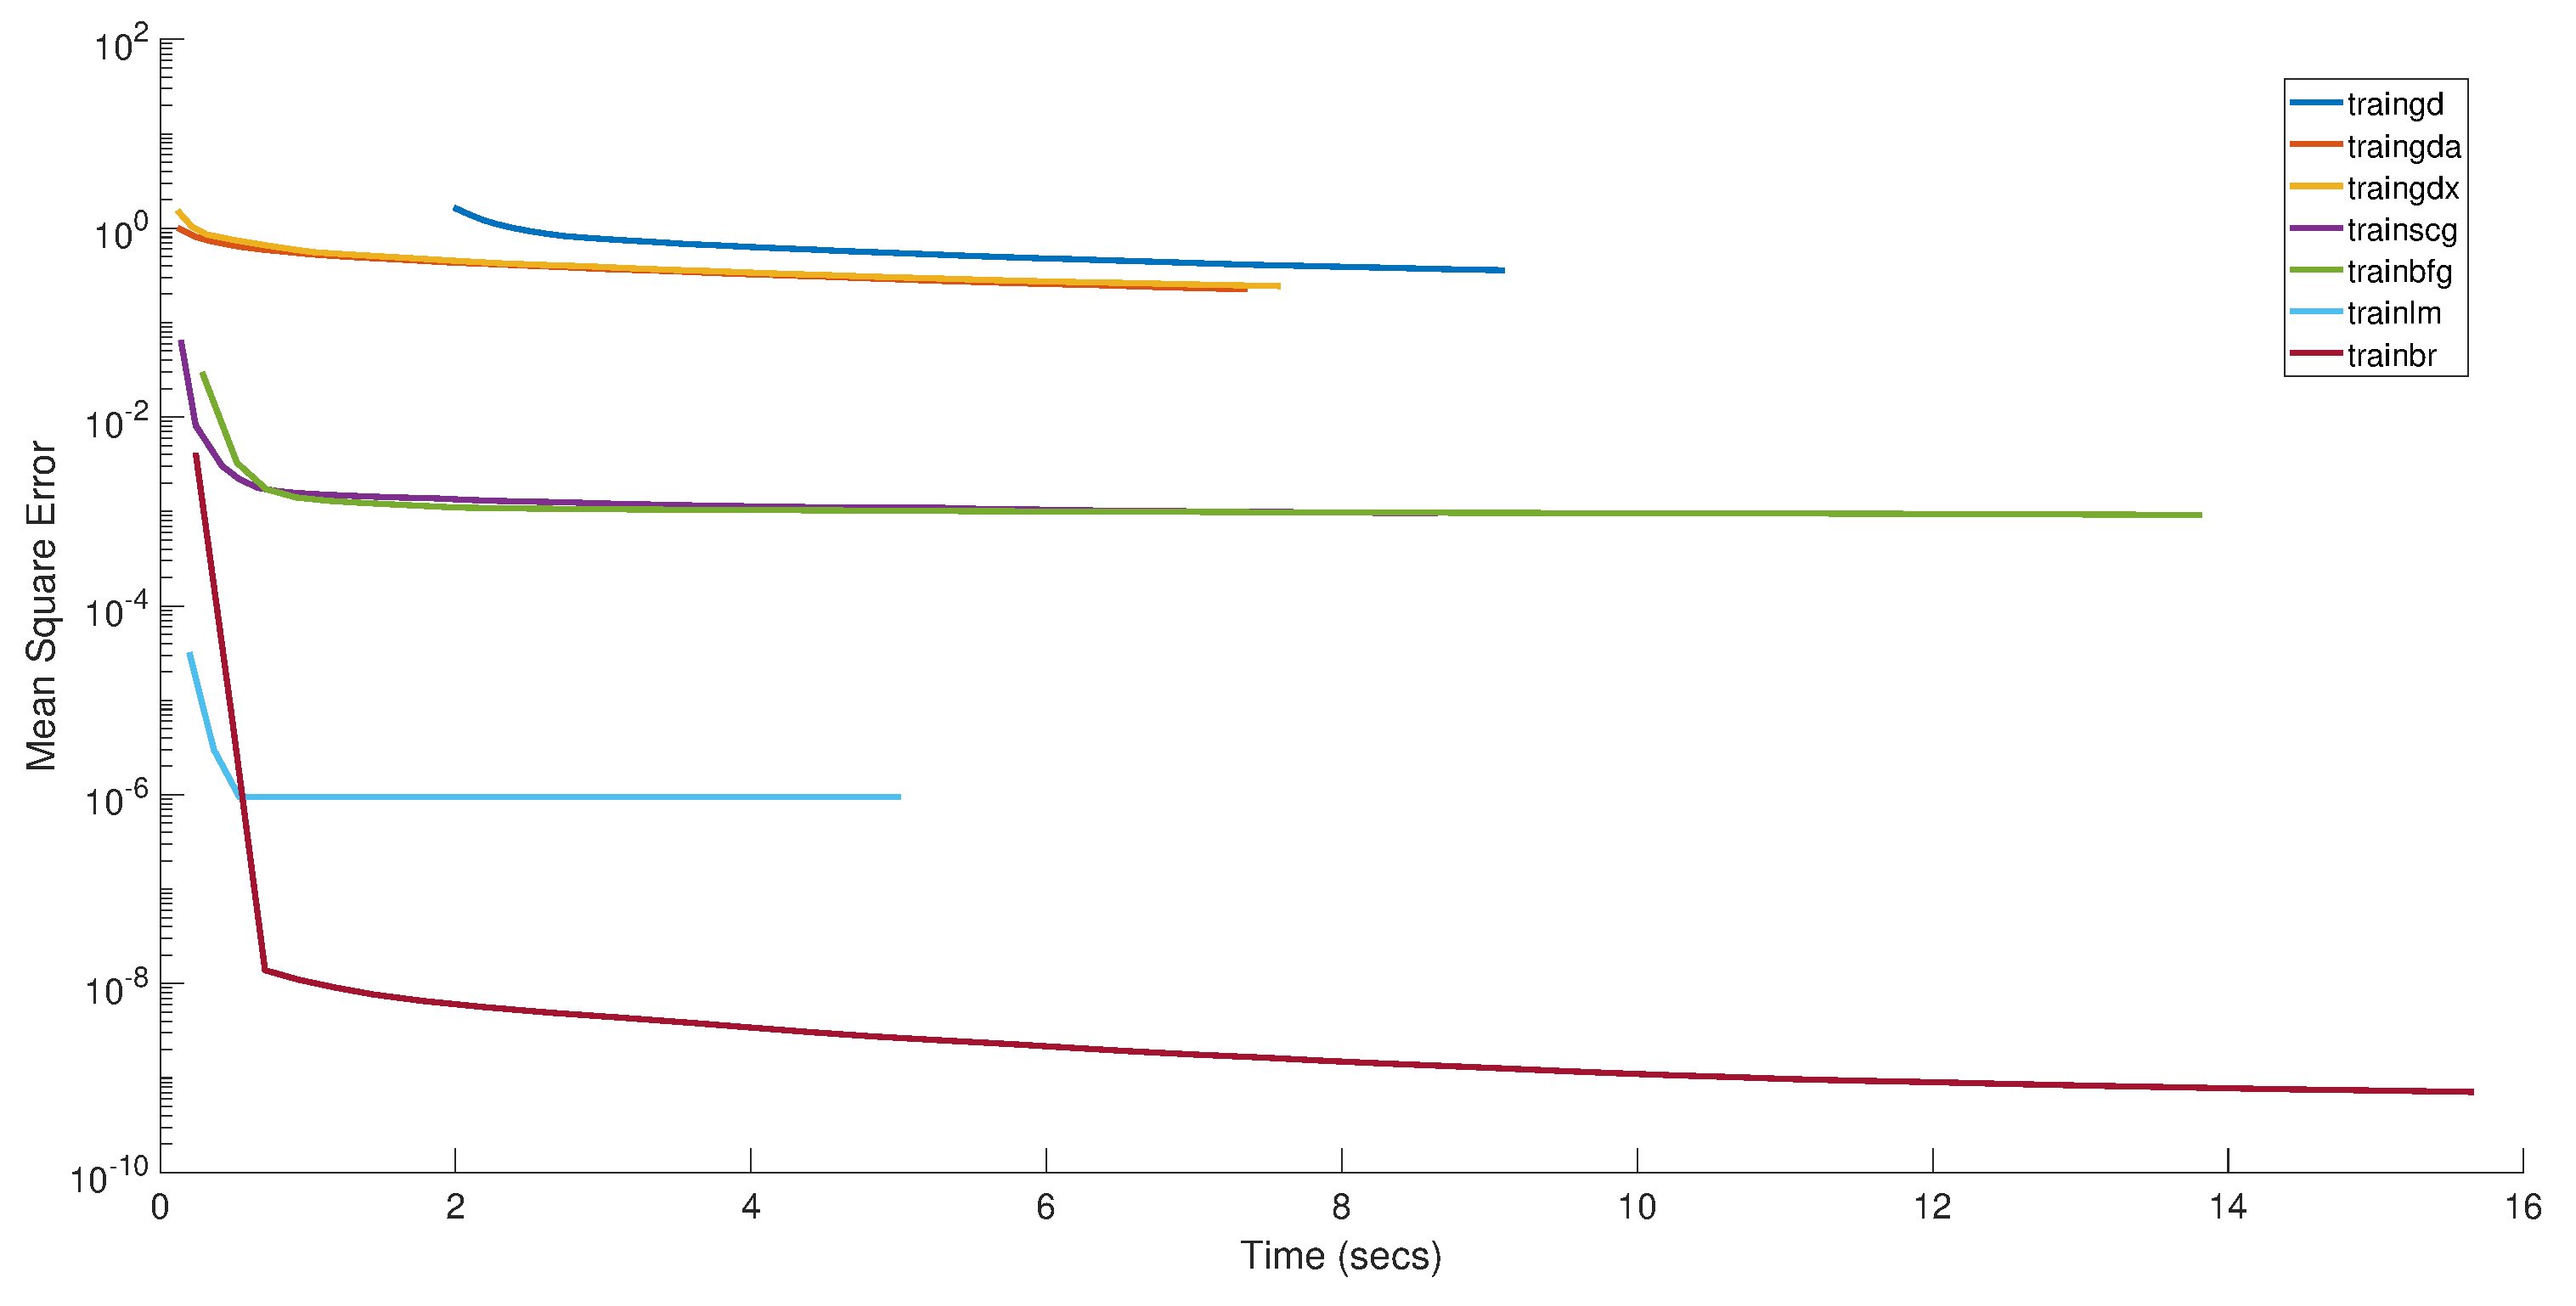
\includegraphics[height = 0.7\textwidth,width = 1\textwidth]{Exercise1/Report/mse_2_noise}
		\caption{MSE VS Training time \newline}\label{fig:mse_2_noise}
	\end{subfigure}
	\captionsetup{format = hang}
	\caption{Performance of various training algorithms on input data with noise}
	\label{fig:train_perf_noise}
\end{figure}
From figure \ref{fig:mse_1_noise} it can be seen that both Levenberg-Marquardt with Bayesian regularization \textit{(trainbr)} and Levenberg-Marquardt \textit{(trainlm)} gives smaller mean square errors but Levenberg-Marquardt is faster as it takes lesser time for convergence of the mean the error over 1000 epoch as shown in figure \ref{fig:mse_2_noise}.
\section{Personal regression}
In this exercise we try to approximate an unknown non-linear function on a dataset with 136000 points. We only consider the first 3000 data points to create our train, validation and test sets. We randomly permutate the data points and chose 1000 points amongst the dataset for each of train, validation and test sets.The target data points is generated as $T_{new} = (8T1+7T2+7T3+6T4+ 3T5)/(8+7+7+6+3)$. The train and validation scatter plots on a mesh grid is shown in the figure \ref{fig:data}. For training the model we use both training and validation data sets. We train the model with [20 50 100] neuron combinations in the hidden layers using various training algorithms and transfer functions. Out of these models, we chose the model with best performance and least mean square error to predict the approximations on the test dataset. Some of the results of the training methods is given in the table

\begin{figure}[!htpb]
	\centering
	\begin{subfigure}[b]{0.5\textwidth}
		\captionsetup{width=0.8\linewidth, format = hang}
		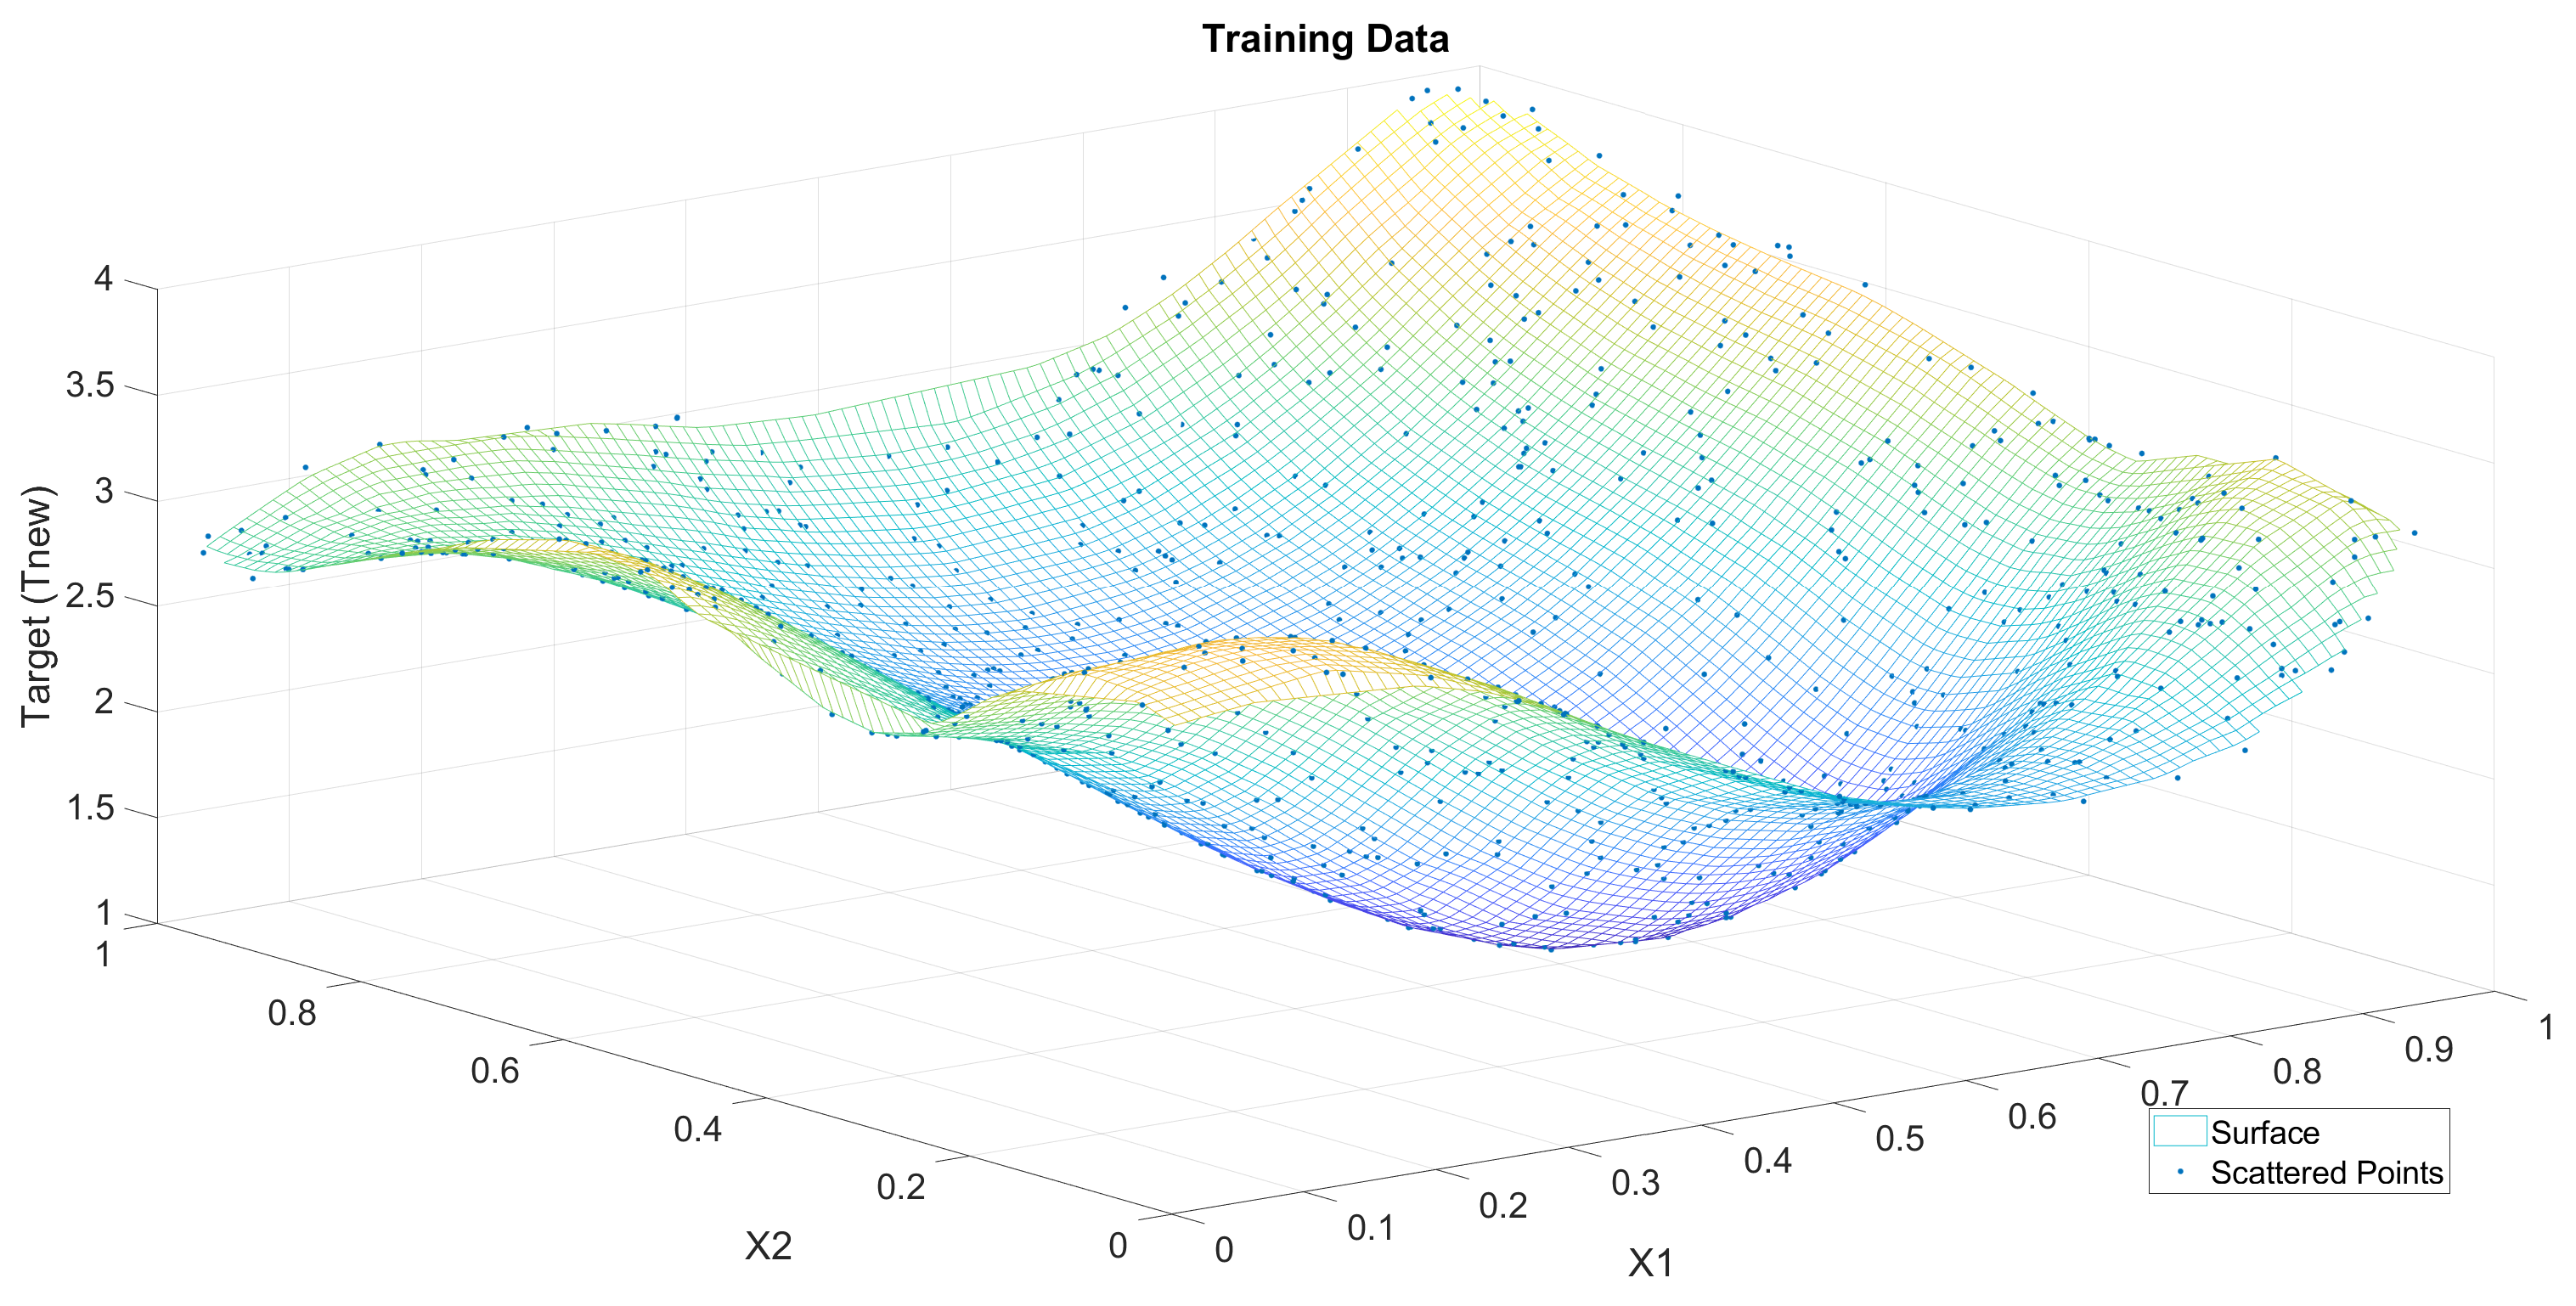
\includegraphics[height = 0.6\textwidth,width = 1\textwidth]{Exercise1/Report/pers_reg_train}
		\caption{Training data points }\label{fig:train}
	\end{subfigure}%
	\begin{subfigure}[b]{0.5\textwidth}
		\captionsetup{width=0.8\linewidth, format = hang}
		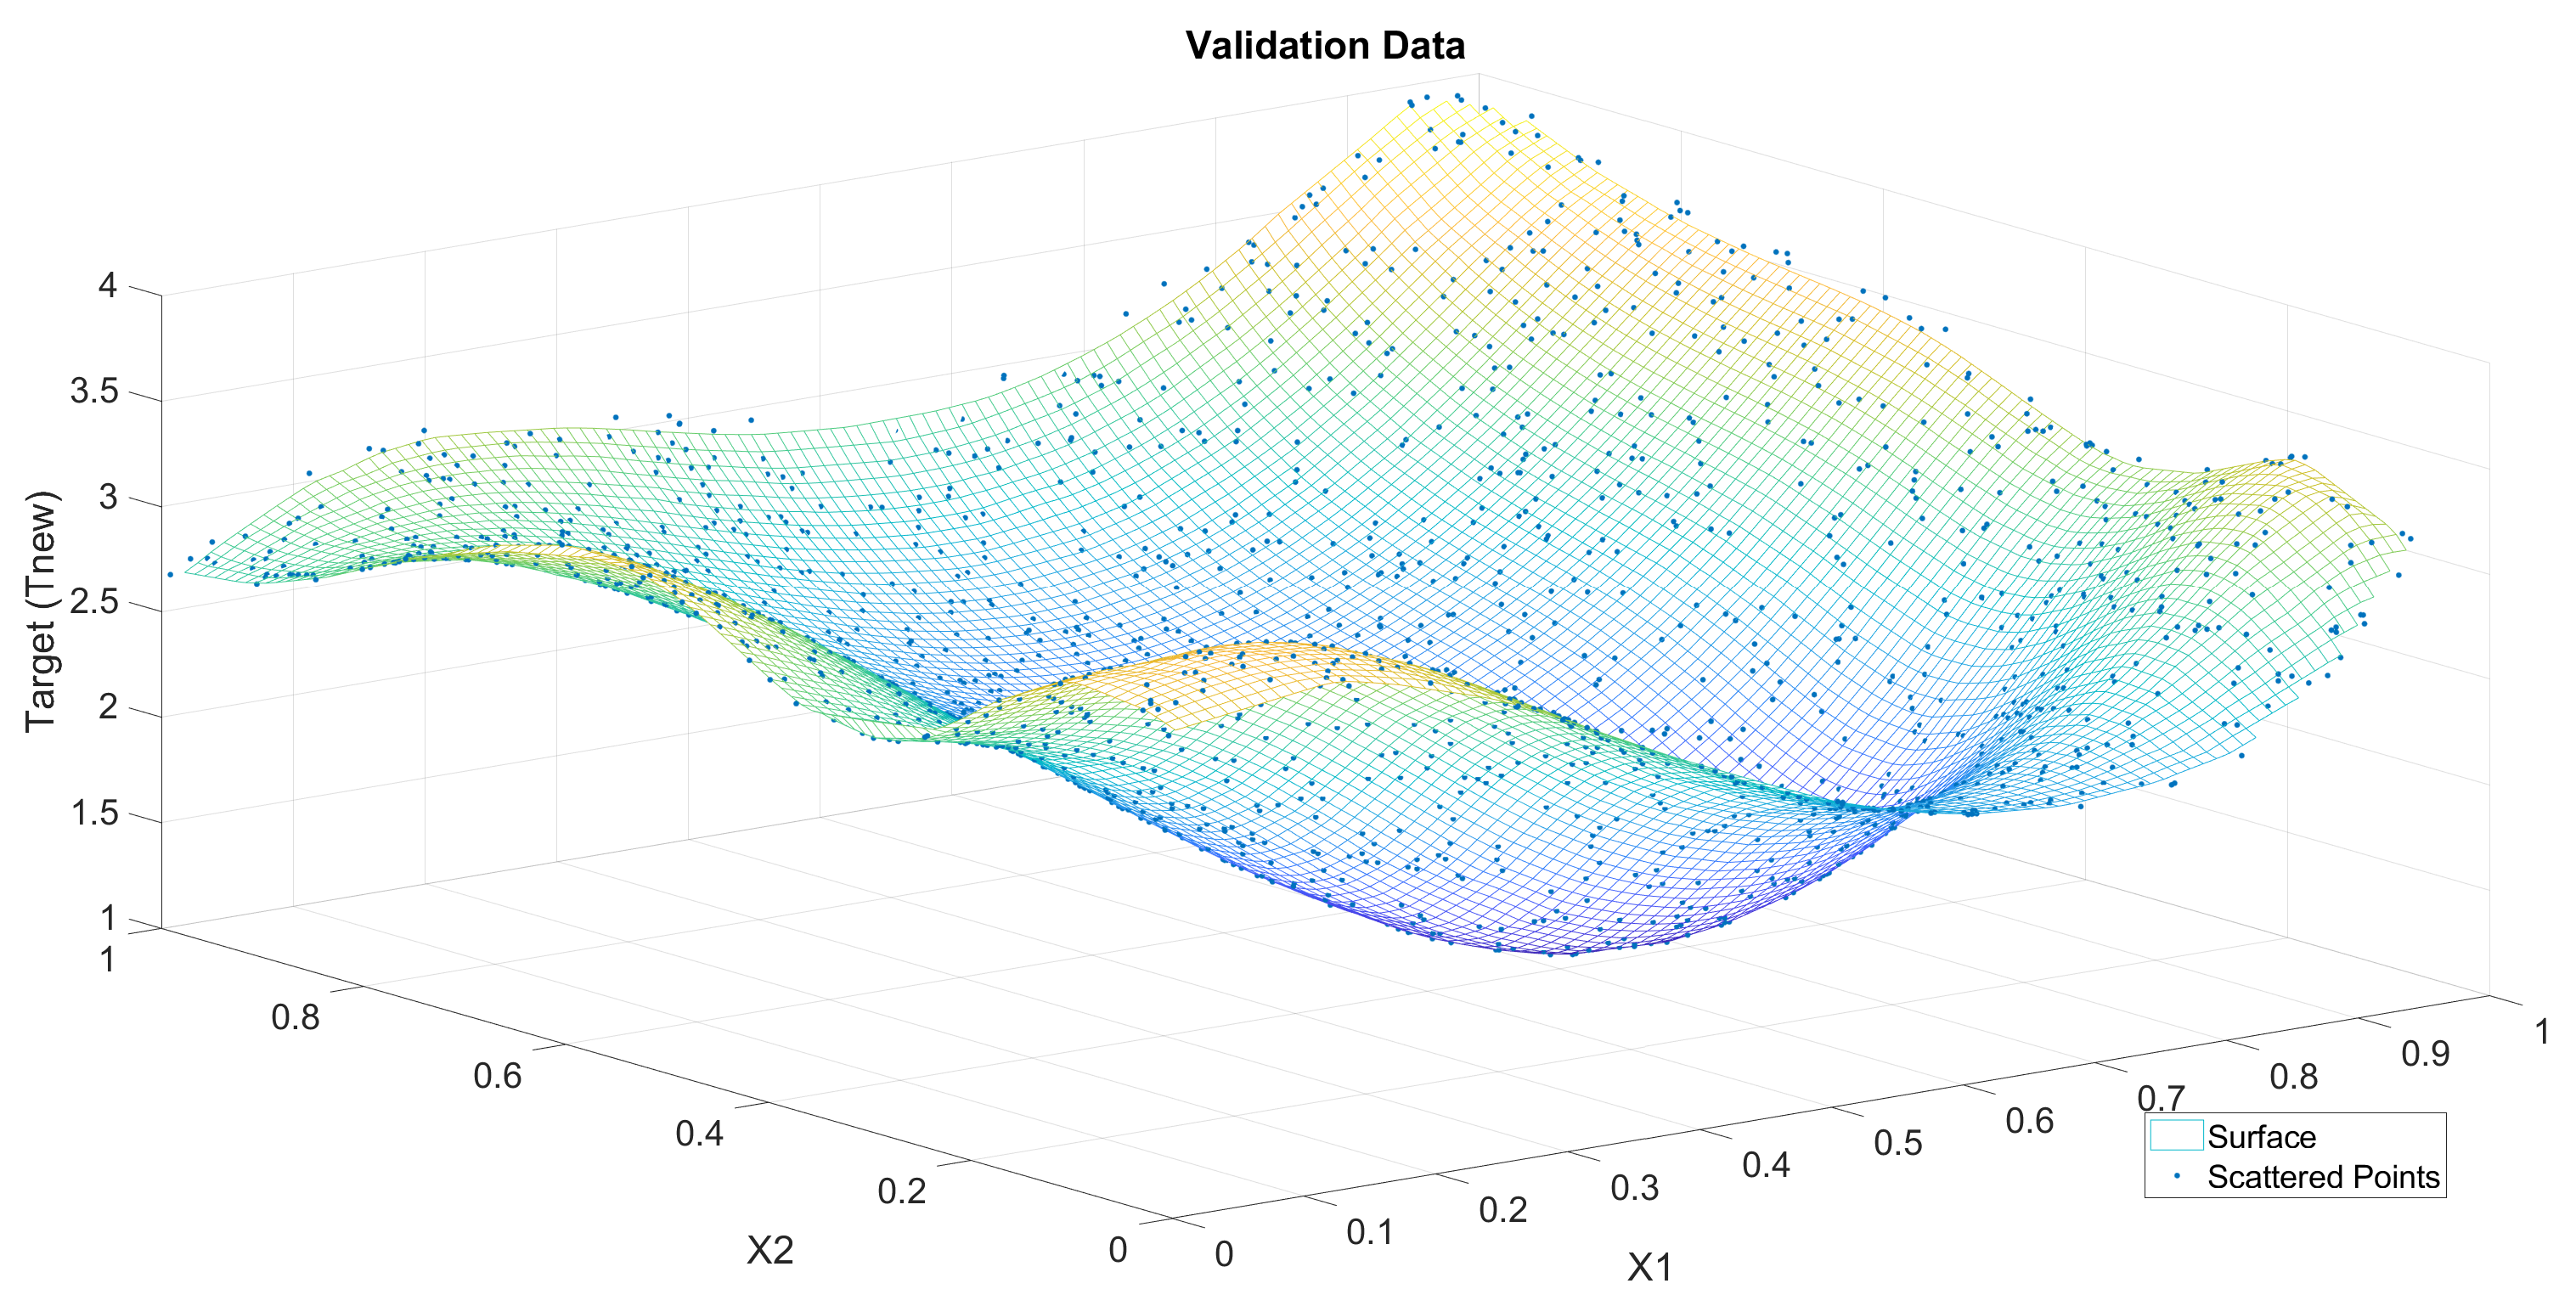
\includegraphics[height = 0.6\textwidth,width = 1\textwidth]{Exercise1/Report/pers_reg_val}
		\caption{Validation data points}\label{fig:val}
	\end{subfigure}%
	\caption{Scatter and Mesh plots of Training and validation data points}
	\label{fig:data}
\end{figure}

\begin{table}[!htpb]
	\centering
	\begin{tabular}[t]{|>{\centering}p{2cm}|p{2cm}|p{2cm}|p{2cm}|p{2cm}|p{2cm}|}
		
		\cellcolor{blue!25}Training Algorithm & \cellcolor{blue!25} Network transfer function& \cellcolor{blue!25}Hidden units  & \cellcolor{blue!25} MSE on train set & \cellcolor{blue!25} MSE on val set & \cellcolor{blue!25} Training Time\\ \hline
		traingd &  logsig& 20 & 0.065107 & 0.063997 & 4.3129 \\ \hline
		traingd &  tansig& 20 & 0.040031 & 0.040949 & 4.2408 \\ \hline
	
		trainlm &  logsig& 50 & 8.645e-07 & 4.8764e-06 & 36.538 \\ \hline
		trainlm &  tansig& 50 & 1.4024e-06 & 4.6243e-06 & 6.6497 \\ \hline			
	
		trainbr &  logsig& 50 & 2.233e-09 &1.2061e-08 & 42.345 \\ \hline
		trainbr &  tansig& 50 & 1.0037e-09 & 1.3104e-08 & 41.626 \\ \hline
		
		trainlm &  tansig& 100 & 5.5275e-09 &1.4636e-07 & 144.04 \\ \hline
		trainbr &  tansig& 100 & 2.805e-10 & 2.2196e-09 & 146.42 \\ \hline
	\end{tabular}
	\captionsetup{format = hang}
	\caption{Performance of a training algorithms in non-linear function approximation of the given data points for various configurations}
	\label{table:1.1} 
\end{table}
From the table \ref{table:1.1} it can be seen that both \textit{trainlm} and \textit{trainbr} algorithms gives smaller MSE's on train and validations.  The method \textit{trainlm} with 50 hidden units and \textit{'tansig'} network transfer function takes smaller training time. The MSE of this configuration is less and acceptable even though \textit{trainbr} has the minimum value. Therefore, we test our test set with this configuration for the non-linear function approximation. The predictions on the test set is shown in the figure \ref{fig:test_out}. It can be noticed that the model performs at its best. To further improve the performance, we can tune the hyper parameters and use more hidden layers and hidden units with drop out nodes (to avoid over fitting).

\begin{figure}[!htpb]
	\centering
	\captionsetup{format = hang}
	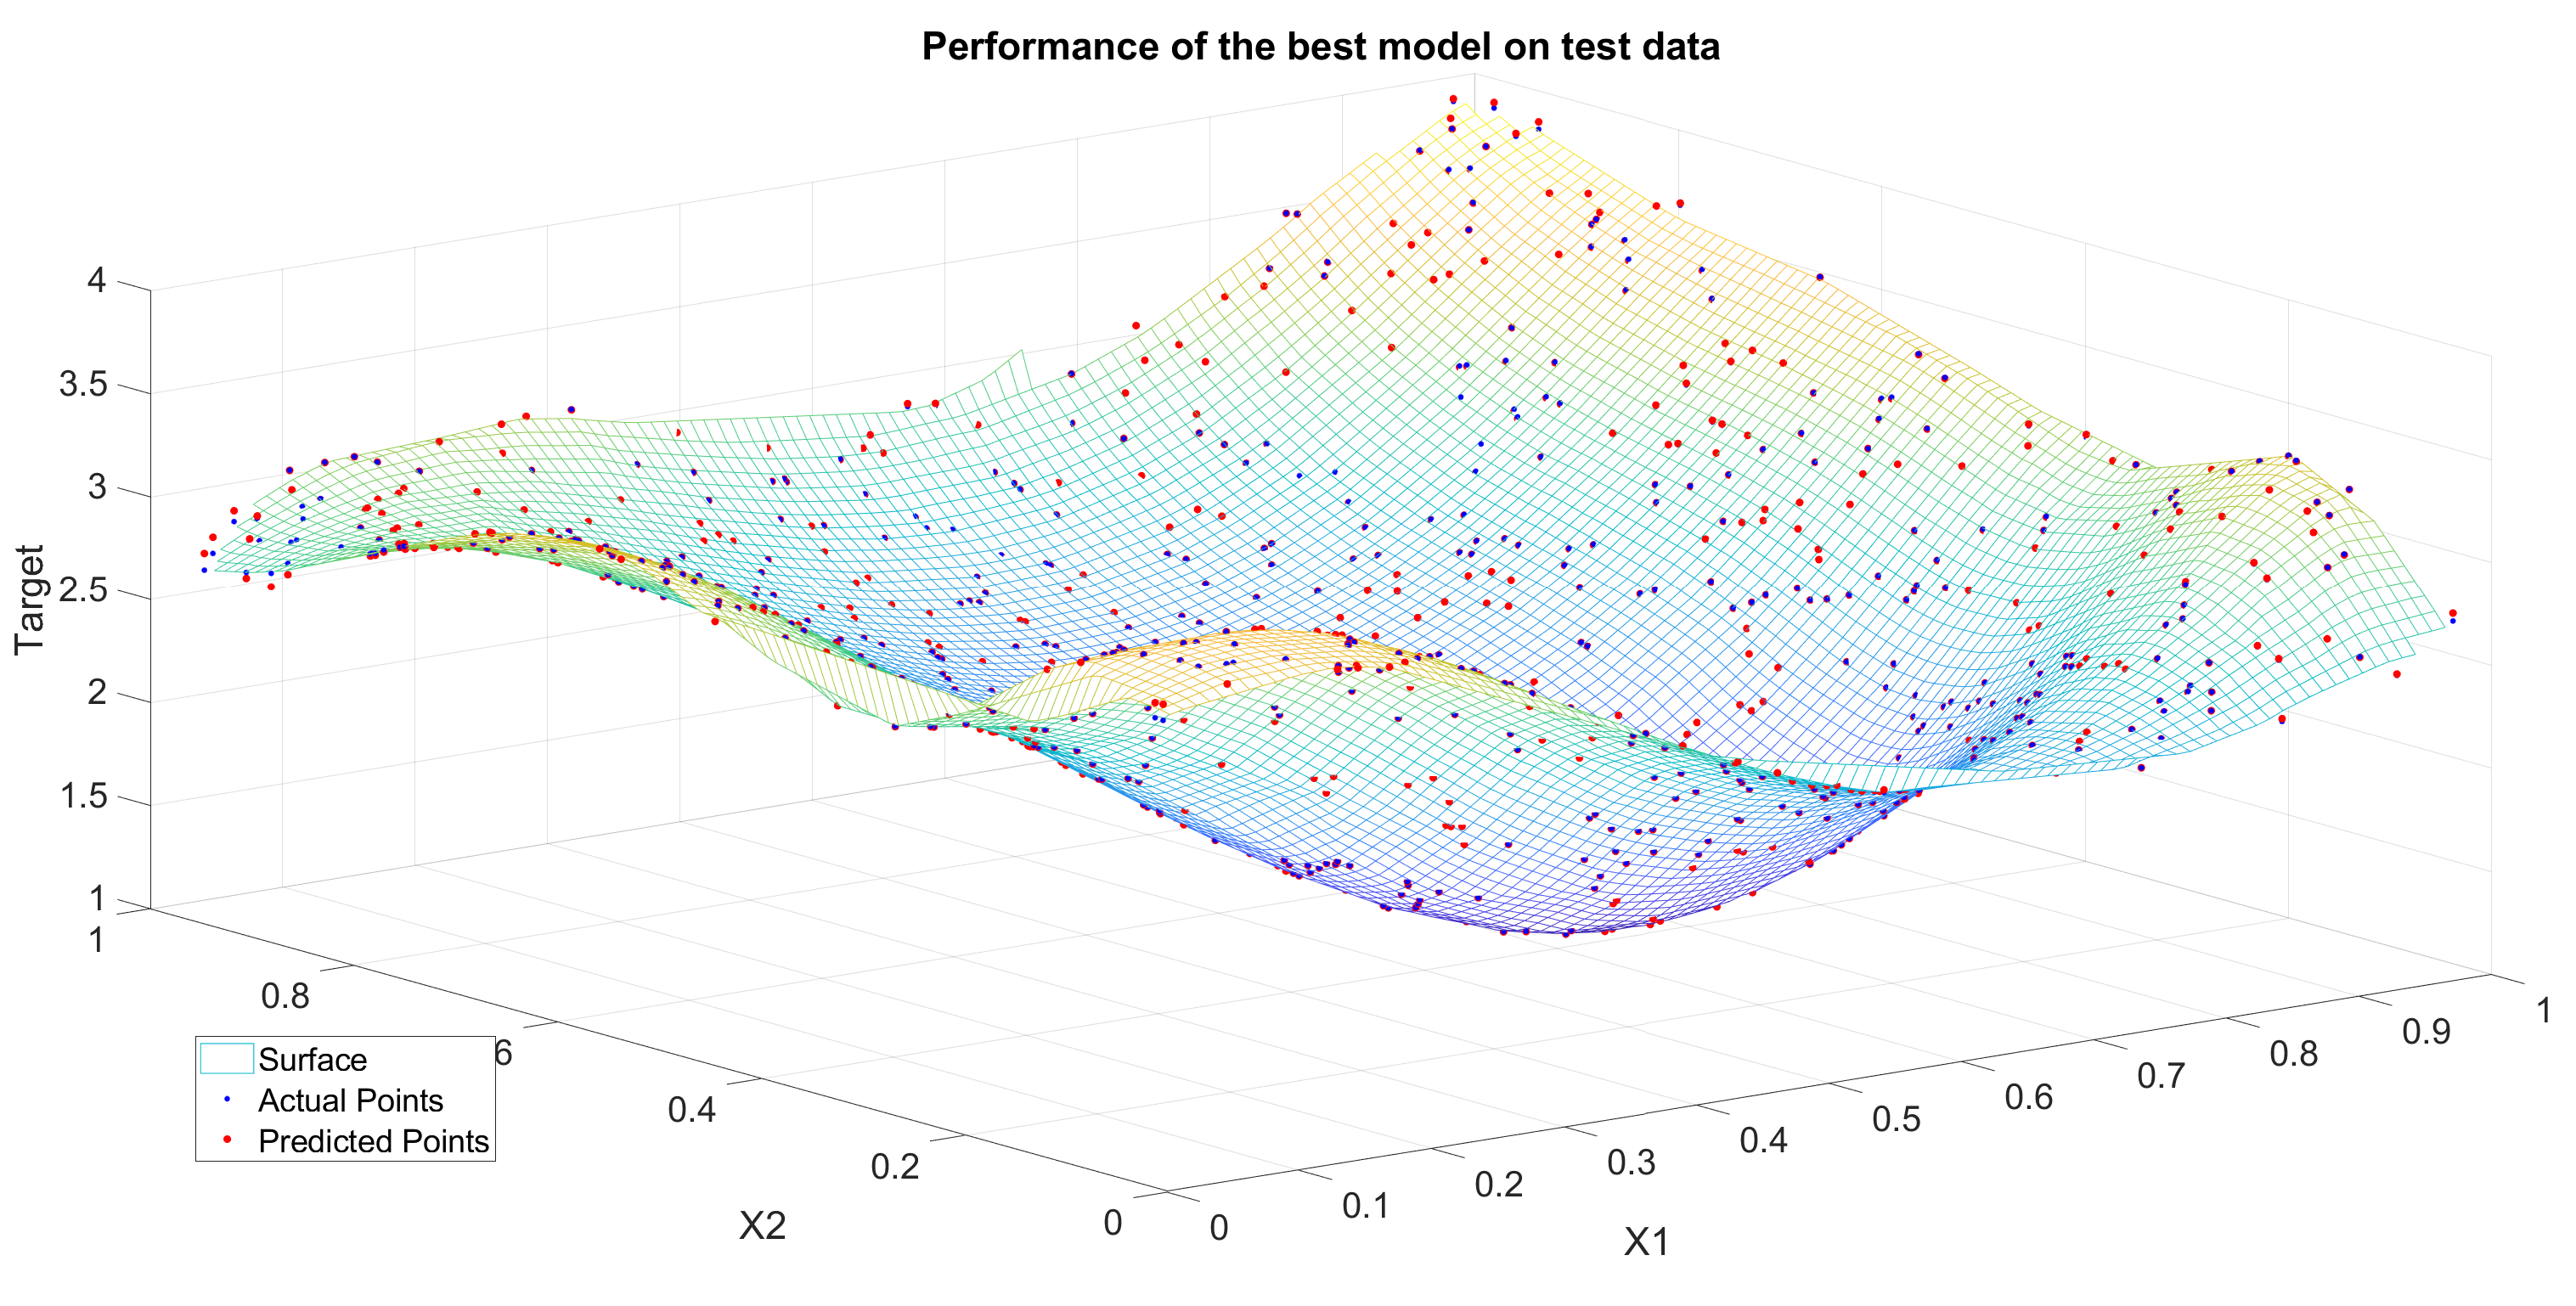
\includegraphics[width = 0.8\textwidth]{Exercise1/Report/test_out}
	\caption{Non linear function approximates on test set} \label{fig:test_out}
\end{figure}

\section{Bayesian Inference}
\begin{table}[!htpb]
	\captionsetup{format = hang}
	\caption{Performance of training algorithms for input data with and without noise}
	\label{table:1.2} 
\begin{subtable}{.52\linewidth}
	\centering
	\caption{Performance on data without noise \newline}\label{table:1.2.1}
	\begin{tabular}[t]{|>{\centering}p{1.8cm}|p{1.1cm}|p{2cm}|p{1.6cm}|}
	\cellcolor{blue!25}Training Algorithm & \cellcolor{blue!25}Hidden units  &  \cellcolor{blue!25} MSE on training set	 & \cellcolor{blue!25} Training Time	 \\ \hline
{'traingd' }    &   30       &    0.41024     &   1.4715  \\ \hline
{'traincgf'}    &   30       &    0.11332    &   2.9307 \\ \hline
{'trainlm' }    &   30       &    0.049307  &   3.0955\\ \hline
{'trainbr' }    &   30       &    0.00016628     &   6.111\\ \hline
{'traingd' }    &   50       &    0.22564     &   2.1072\\ \hline
{'traincgf'}    &   50       &    0.021669    &   3.8808\\ \hline
{'trainlm' }    &   50       &    1.9356e-09  &   6.6776\\ \hline
{'trainbr' }    &   50       &    5.8591e-11  &   9.4141\\ \hline
{'traingd' }    &   100      &    0.28868     &   2.5079\\ \hline
{'traincgf'}    &   100      &    0.000343 &   4.3097\\ \hline
{'trainlm' }    &   100      &    2.9575e-16  &   0.94997\\ \hline
{'trainbr' }    &   100      &    5.8841e-11  &   5.4633\\ \hline
{'traingd' }    &   150      &    0.28617     &   2.4044\\ \hline
{'traincgf'}    &   150      &    2.3958e-05  &   2.9279\\ \hline
{'trainlm' }    &   150      &    9.2161e-17  &   0.21211\\ \hline
{'trainbr' }    &   150      &    4.9838e-06  &   39.717\\ \hline
	\end{tabular}
	\end{subtable}%
\begin{subtable}{.52\linewidth}
	\centering
	\caption{Performance on noisy data with noise level $\sigma = 0.5$ (standard deviation) }\label{table:1.2.2}
	\begin{tabular}[t]{|>{\centering}p{1.8cm}|p{1.1cm}|p{2cm}|p{1.6cm}|}
		\cellcolor{blue!25}Training Algorithm & \cellcolor{blue!25}Hidden units  & \cellcolor{blue!25} MSE on training set	 & \cellcolor{blue!25} Training Time	 \\ \hline
		{'traingd' }    &   30      &    0.45688     & 1.2805 \\ \hline
		{'traincgf'}    &   30      &    0.25429     & 2.3445 \\ \hline
		{'trainlm' }    &   30      &    0.12776     & 2.4669\\ \hline
		{'trainbr' }    &   30      &    0.1832      & 3.1289\\ \hline
		{'traingd' }    &   50      &    0.32496     & 1.1241\\ \hline
		{'traincgf'}    &   50      &    0.14655     &   2.6011\\ \hline
		{'trainlm' }    &   50      &    0.067438    &   3.8249\\ \hline
		{'trainbr' }    &   50      &    0.12235     &   4.9785\\ \hline
		{'traingd' }    &   100     &    0           &  0.31386\\ \hline
		{'traincgf'}    &   100     &    0.028183    &   3.3844\\ \hline
		{'trainlm' }    &   100     &    0.00016868  &   6.6878\\ \hline
		{'trainbr' }    &   100     &    0.0036395   &   9.5772\\ \hline
		{'traingd' }    &   150     &    0           &  0.34608\\ \hline
		{'traincgf'}    &   150     &    0.0064246   &   4.1436\\ \hline
		{'trainlm' }    &   150     &    2.5763e-27  &   10.262\\ \hline
		{'trainbr' }    &   150     &    0.00016898  &   24.427\\ \hline
	\end{tabular}
\end{subtable}%	
\end{table}
In this exercise we evaluate the training algorithm \textit{trainbr} i.e., Levenberg-Marquardt with Bayesian regularization similar to section 1 of this exercise. As seen in the earlier section, gradient descent does a poor job compared to other algorithms. Here, we compare the algorithm \textit{trainbr} with others for [30;50;100;150] hidden units in its hidden layer. The results of the models are shown in table \ref{table:1.2} and figure \ref{fig:train_br} respectively. From figure \ref{fig:train_br} it can be noticed that \textit{train\_br} approximates better than \textit{train\_gda}, \textit{train\_cgf} and \textit{train\_cgp} for input data with noise while \textit{train\_lm} approximates better than \textit{train\_br}. It was also noticed that for lesser number of hidden units the \textit{train\_br} model doesn't give good approximates. It works well in the case of input data without noise and gives a very small MSE whereas  for input data with noise, \textit{train\_lm} outperforms all the models both in MSE and training time (results can be seen from table \ref{table:1.2}).
\begin{figure}[!htpb]
	\begin{subfigure}[b]{0.5\textwidth}
		\centering
		\captionsetup{ width=0.8\linewidth, format = hang}
		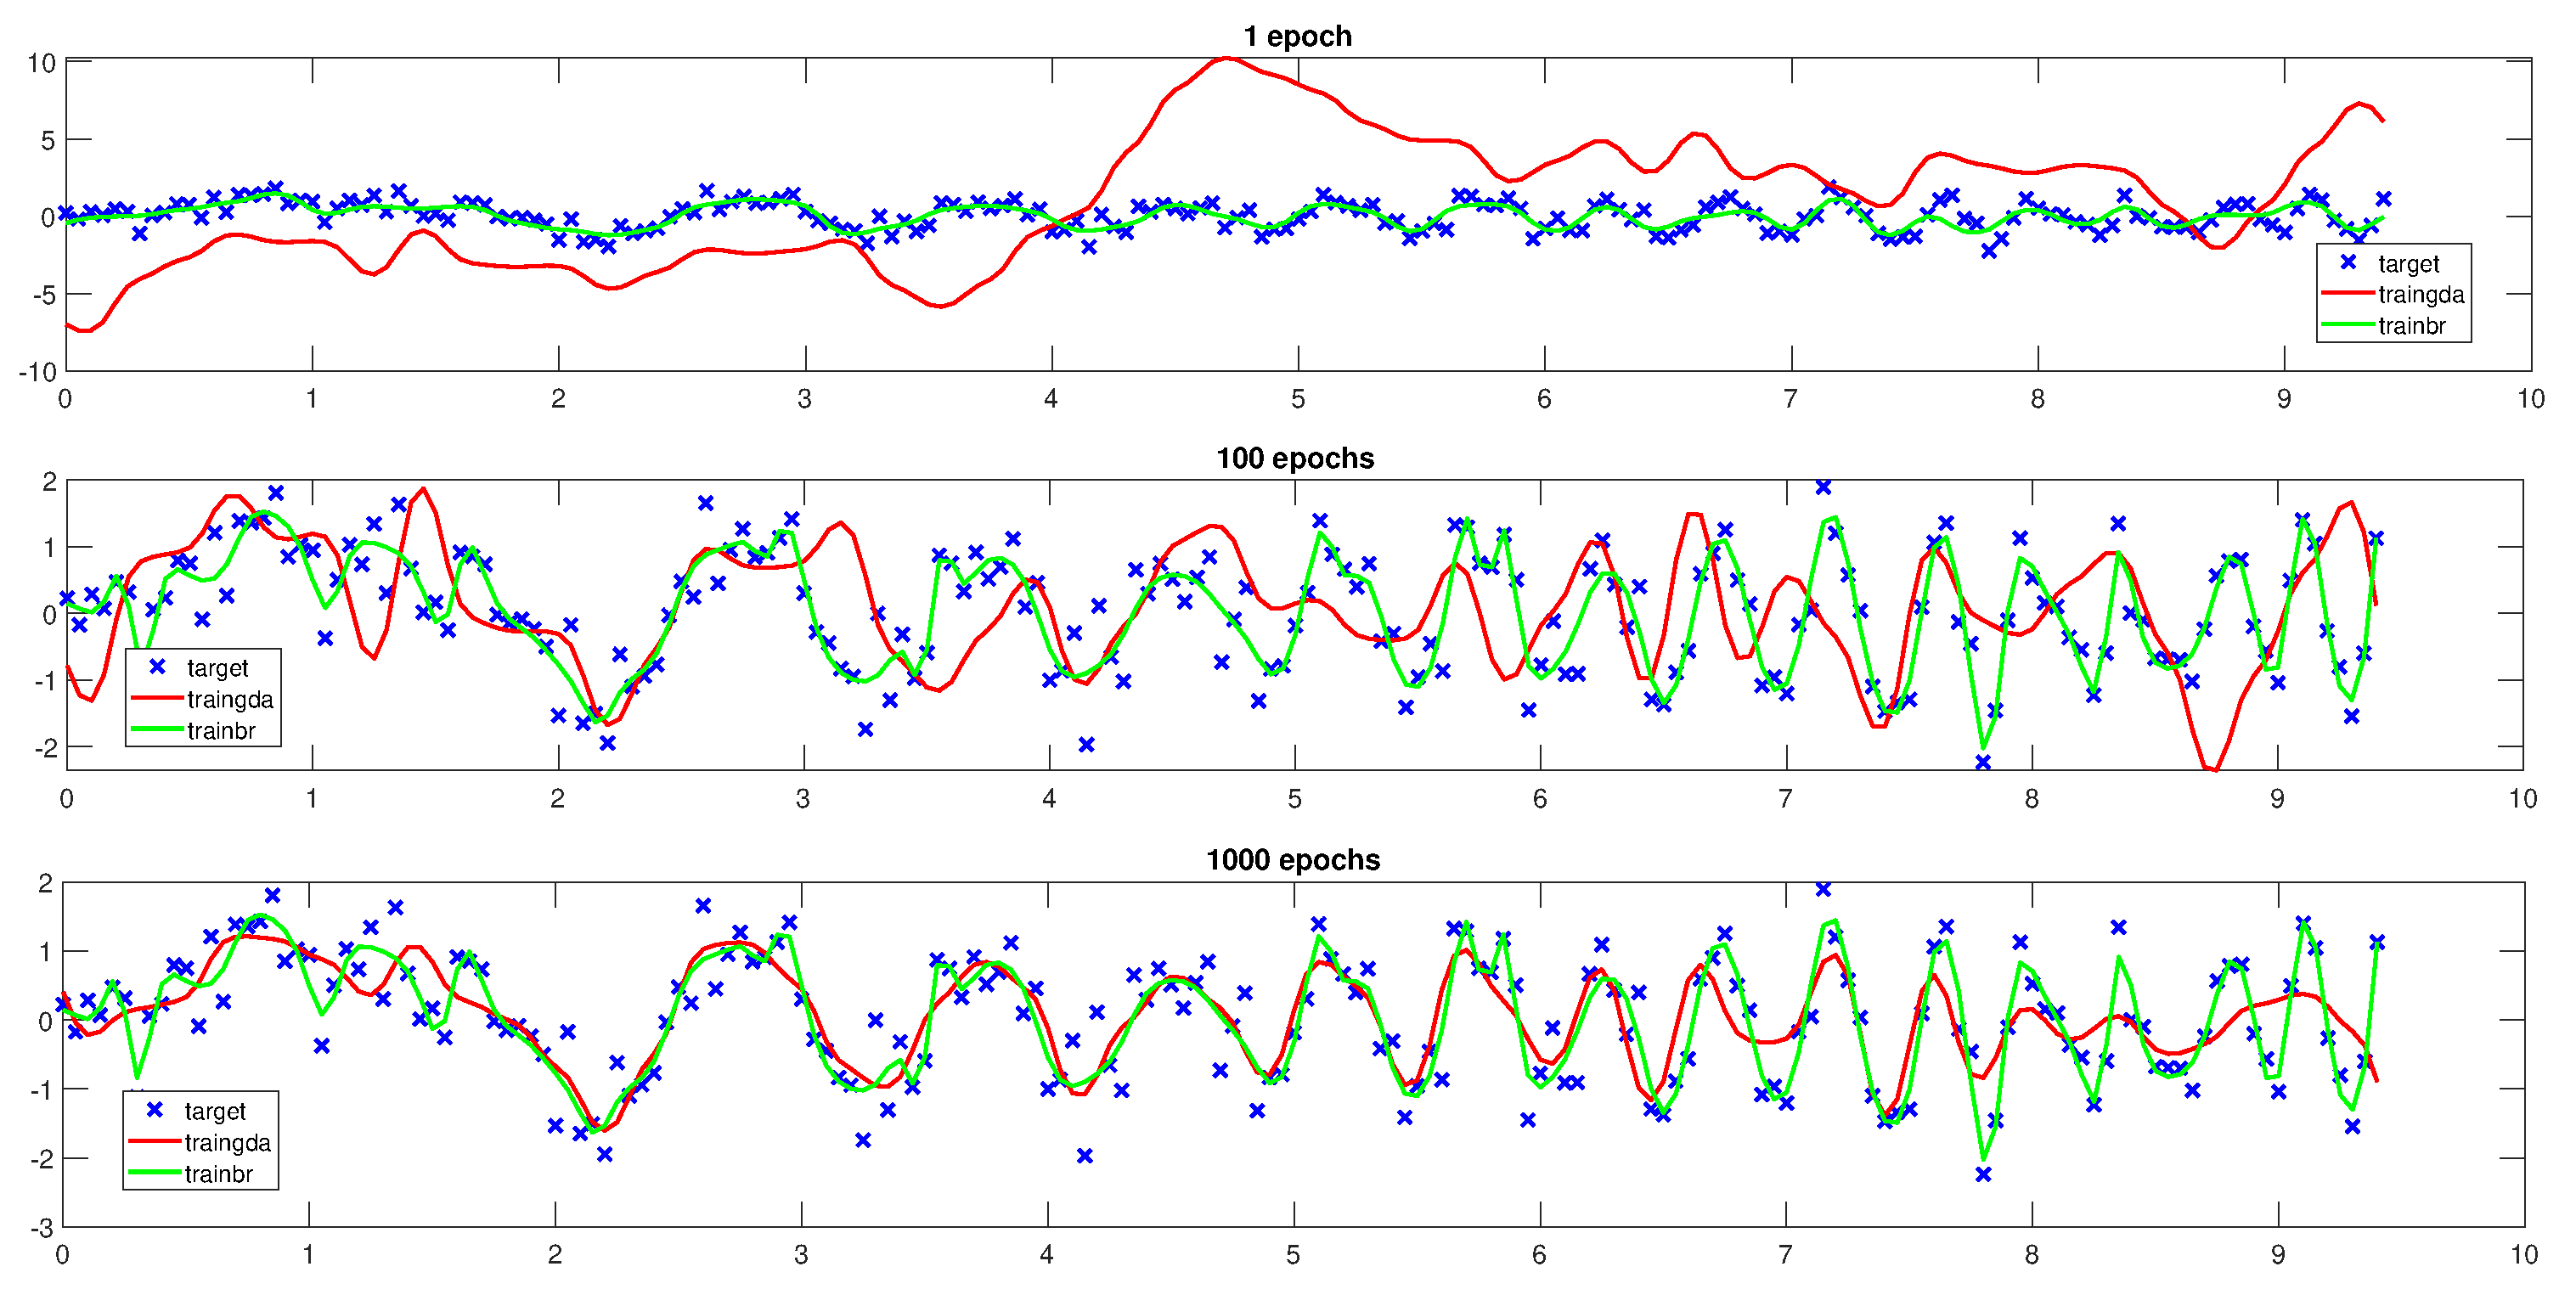
\includegraphics[height = 0.7\textwidth, width = 0.95\textwidth]{Exercise1/Report/train_br_gda}
		\caption{train\_br VS train\_gda}\label{fig:train_br_gda}
	\end{subfigure}%
	\begin{subfigure}[b]{0.5\textwidth}
		\centering
		\captionsetup{width=0.8\linewidth, format = hang}
		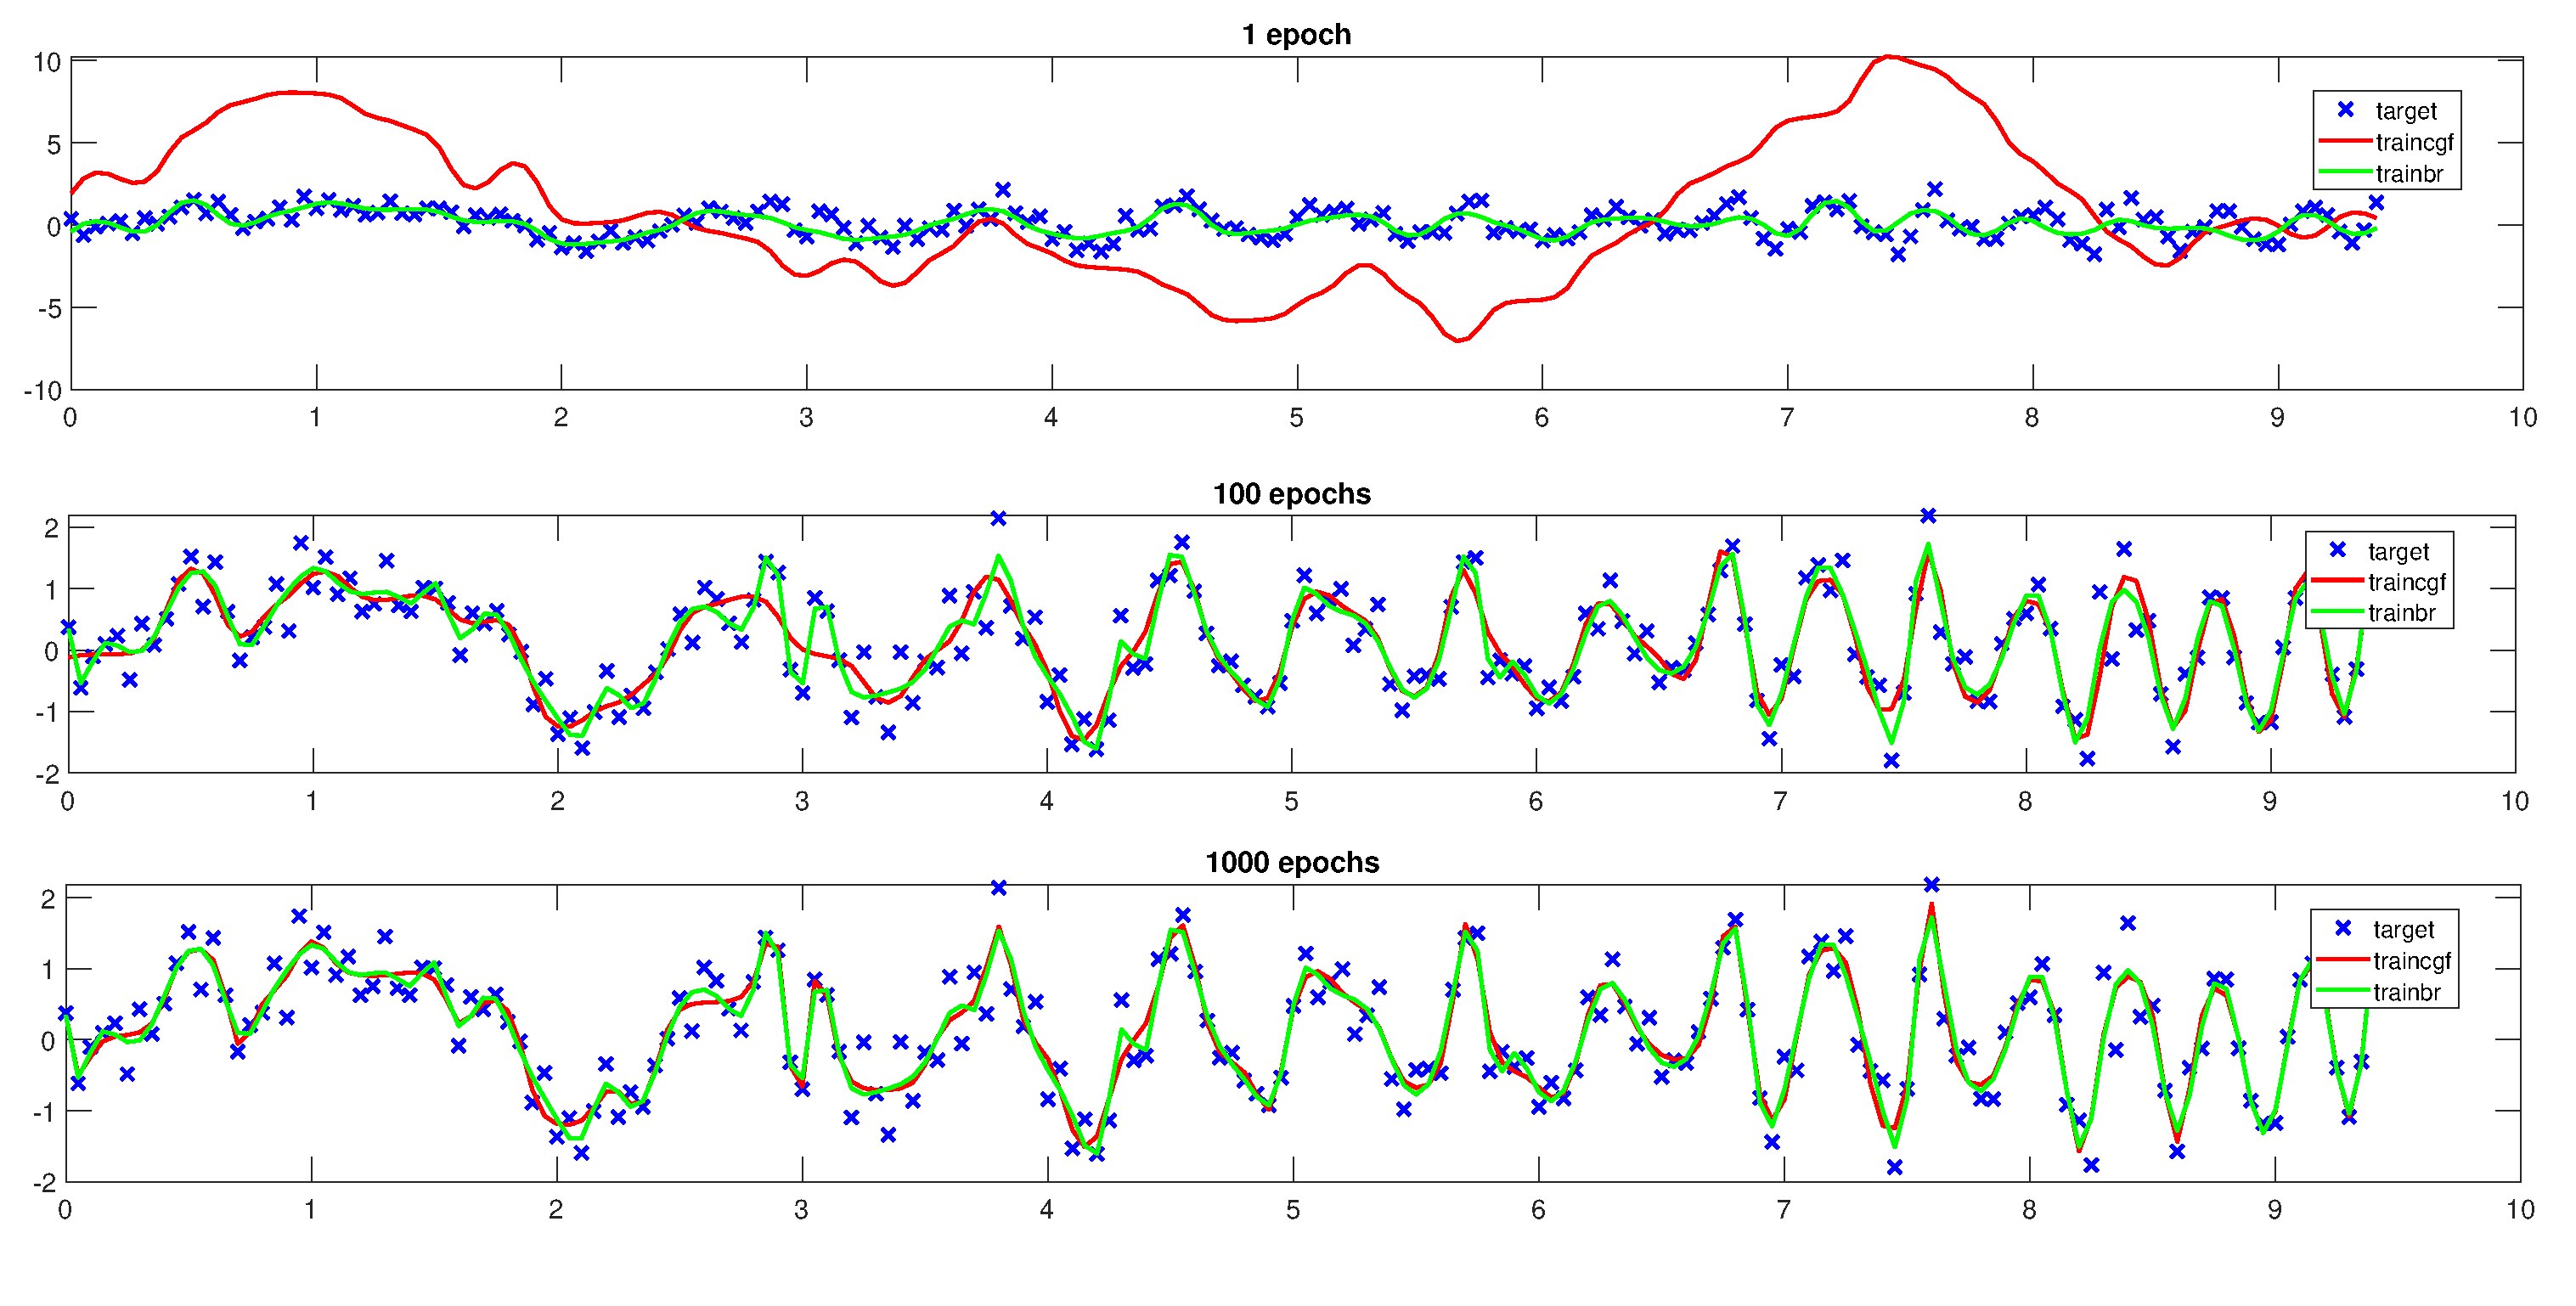
\includegraphics[height = 0.7\textwidth, width = 0.95\textwidth]{Exercise1/Report/train_br_cgf}
		\caption{train\_br VS  train\_cgf}\label{fig:train_br_cgf}
	\end{subfigure}
	\begin{subfigure}[b]{0.5\textwidth}
		\centering
		\captionsetup{width=0.8\linewidth, format = hang}
		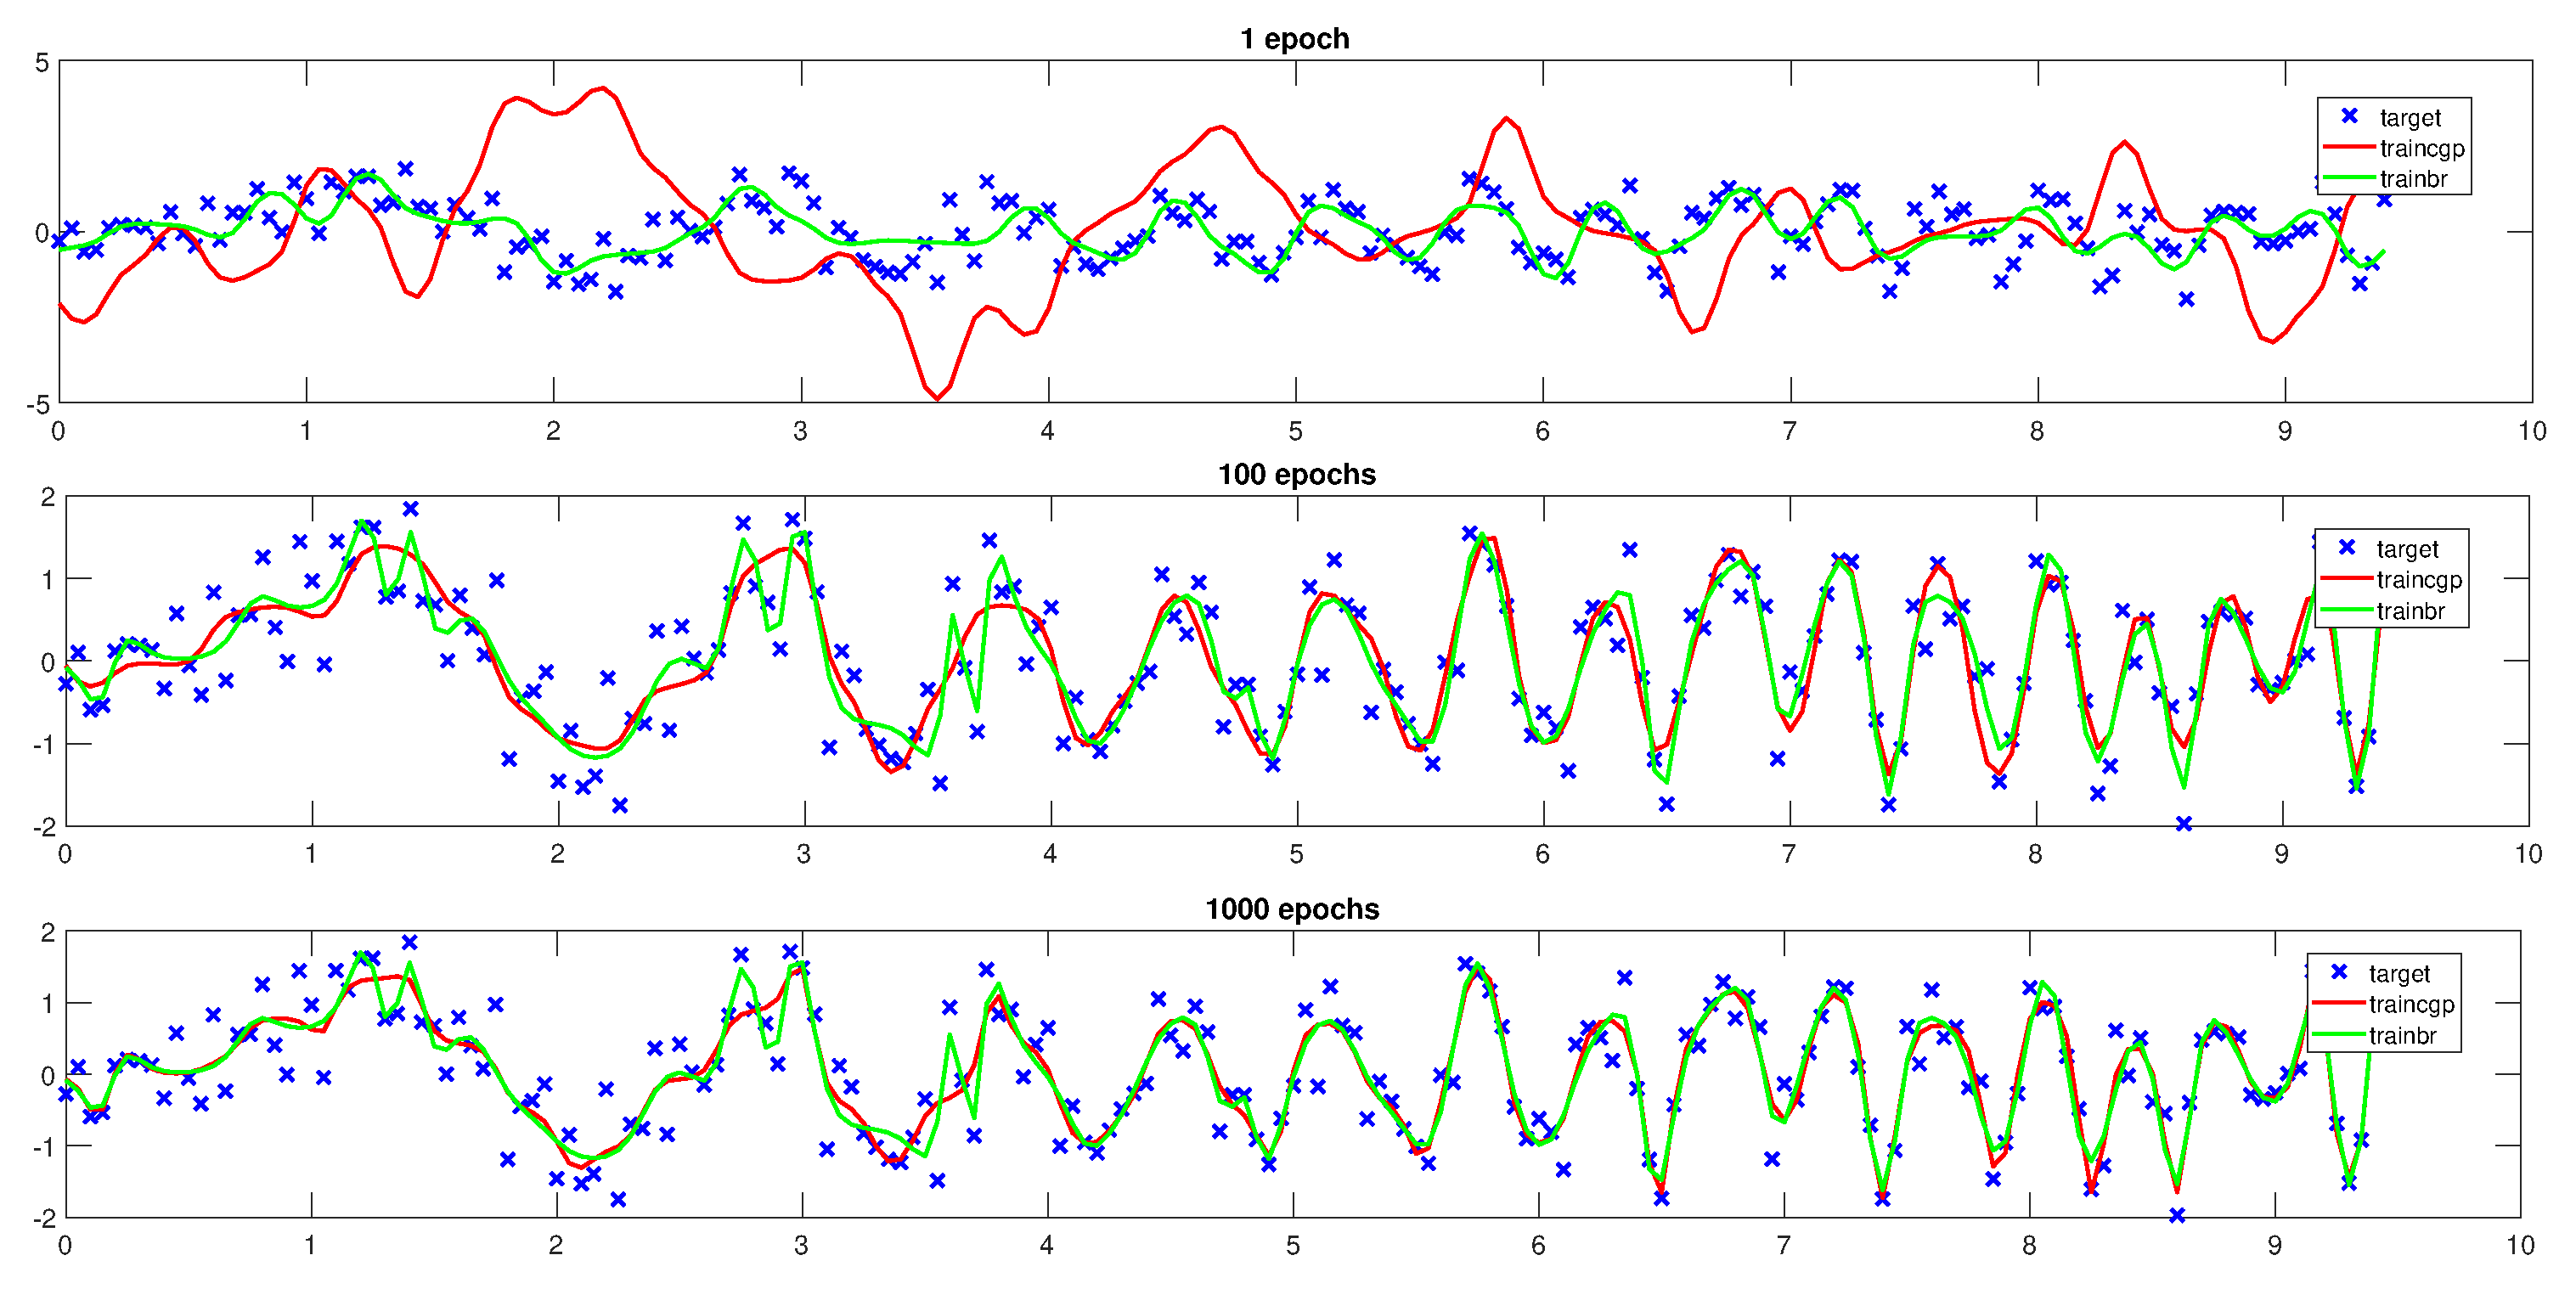
\includegraphics[height = 0.7\textwidth,width = 0.95\textwidth]{Exercise1/Report/train_br_cgp}
		\caption{train\_br VS  train\_cgp}\label{fig:train_br_cgp}
	\end{subfigure}%
	\begin{subfigure}[b]{0.5\textwidth}
		\centering
		\captionsetup{width=0.8\linewidth, format = hang}
		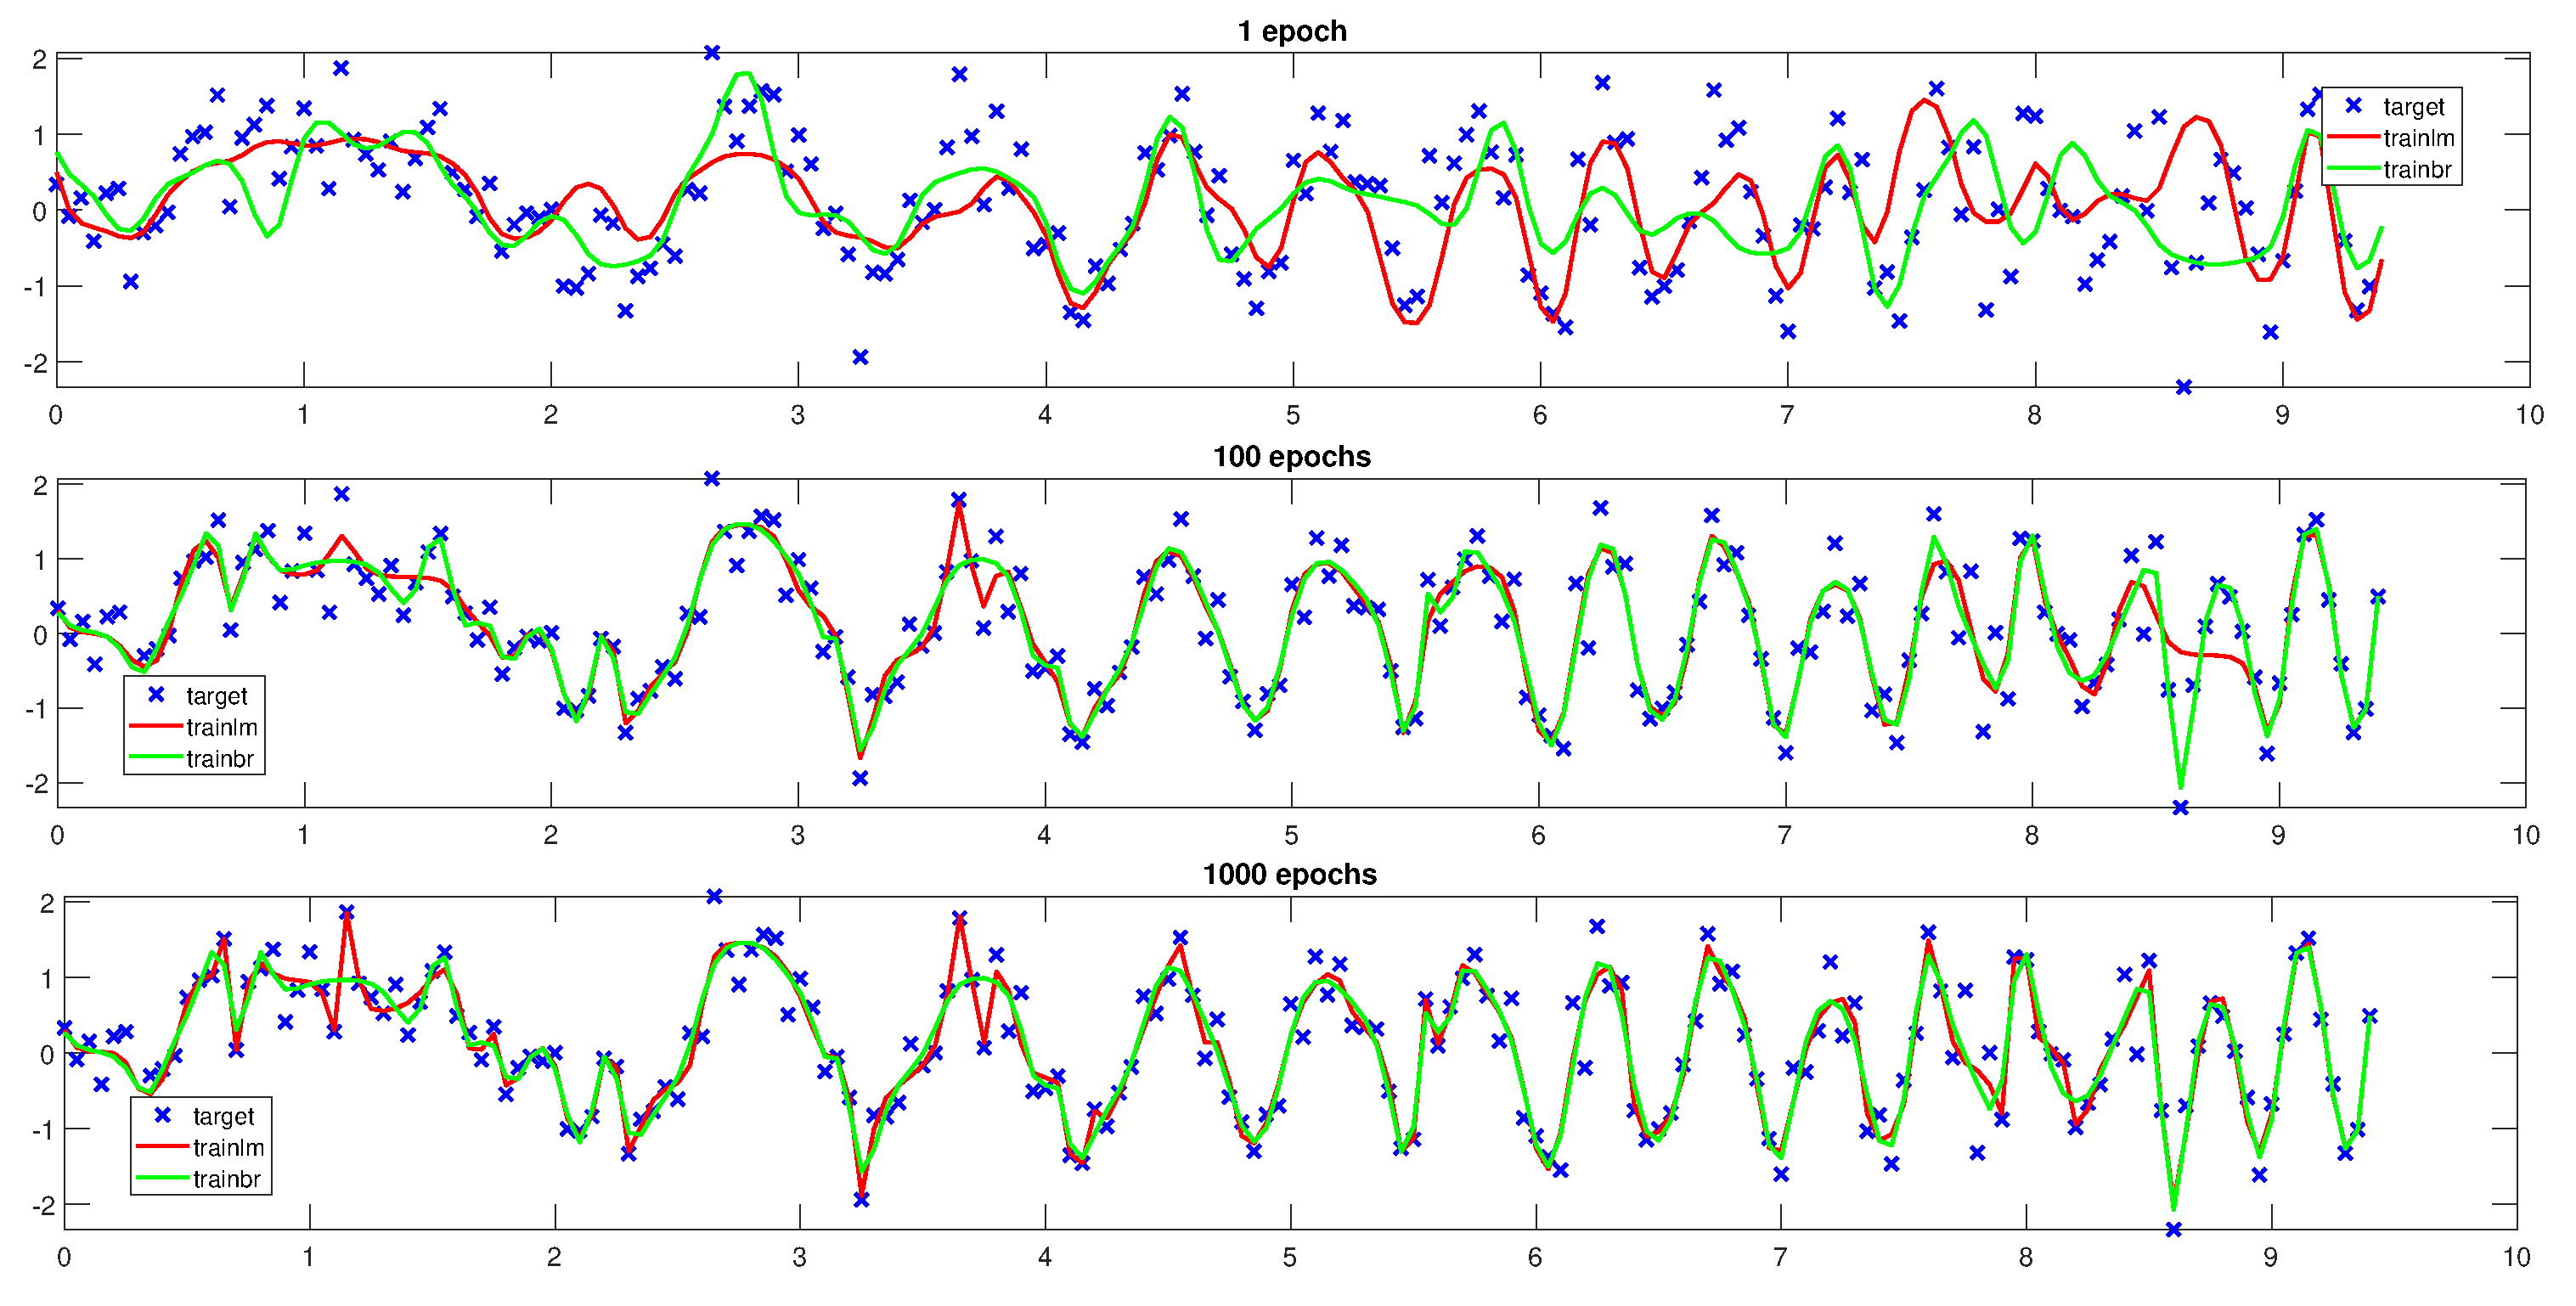
\includegraphics[height = 0.7\textwidth,width = 0.95\textwidth]{Exercise1/Report/train_br_lm}
		\caption{train\_br VS  train\_lm}\label{fig:train_br_lm}
	\end{subfigure}
	\captionsetup{format = hang}
	\caption{Comparison of various training algorithm with \textit{trainbr} on input data for [1;100;1000] epochs}
	\label{fig:train_br}
\end{figure}

Over-parameterized networks take more time to train and the training with more units can only lead to over-fitting. Also, it can be noticed from table \ref{table:1.2} that the overall performance is better for hidden units 50 by taking the training time, MSE, etc. into consideration than with higher number of units like 100 or 150.  